\documentclass[twoside, titlepage, DIV=8, BCOR=8.5mm, open=right, chapterprefix=false]{scrbook}

\usepackage{fontspec}
\usepackage{lmodern} % Remove LaTeX Font Warnings
\usepackage{etoolbox} % programming tools, e.g. newrobustcmd or ifstrequal
\usepackage{csquotes} % fixes warning in polyglossia
\usepackage{polyglossia} % replaces Babel
\usepackage{setspace}
\usepackage[l2tabu, orthodox]{nag} % better warnings
\usepackage{graphicx}
\usepackage{fontawesome} % \faExternalLink
\usepackage{eulervm}       % \AMS Euler math font
\usepackage[normalem]{ulem} % strike-through \sout
\usepackage{marginnote} % \marginpar
\usepackage[natbib, backend=biber, style=authoryear, maxcitenames=2, maxbibnames=99, useprefix]{biblatex}
\usepackage{xcolor} % e.g. for black!50
\usepackage[export]{adjustbox} % for chapter style. Need export for the "inner" option in \includegraphics
\usepackage[section]{placeins}
\usepackage{tikz}
\usepackage{booktabs}
\usepackage{longtable}
\usepackage{tabu}
\usepackage{caption}
\usepackage{relsize}
\usepackage[macros,xspace]{acro} % acronyms (i.e. abbreviations)
\usepackage{hyperref}
\RequirePackage[nameinlink, noabbrev]{cleveref} % load last !!!


% Silencing output from xetex:
\hfuzz=999pt    % reduce overfull hbox errors
\hbadness=10000 % reduce underfull hbox errors
\usepackage{silence}
\WarningFilter{latex}{Marginpar on page}


% Good style recommondations from here:
% https://tex.stackexchange.com/questions/9533/what-best-combination-of-fonts-for-serif-sans-and-mono-do-you-recommend
\setdefaultlanguage[variant=uk]{english}
% https://sourceforge.net/projects/linuxlibertine/. Open Font License
\setmainfont[Mapping=tex-text, Numbers=OldStyle]{Linux Libertine}
% Calibri - looks nice on screen, but not free unfortunately.
% Linux Biolinum O - a bit particular.
% Open Sans - too dense (and line height seems smaller)
\setsansfont[Mapping=tex-text, Numbers=OldStyle]{Linux Biolinum O}
% https://fonts.google.com/specimen/Inconsolata. Open Font License
\setmonofont{Inconsolata}

\addbibresource{references.bib}

\setstretch{1.1}

\graphicspath{{figs/}}


% Chapter style
\renewcommand*\chapterheadstartvskip{\vspace*{0\textheight}}
\renewcommand*\chapterheadendvskip{\vspace*{.1\textheight}}
\setkomafont{chapter}{\rmfamily\fontsize{28}{32}\mdseries}
\makeatletter
\renewcommand*{\@@makechapterhead}[1]{%
    \chapterheadstartvskip
    \noindent
    \begingroup
        \usekomafont{chapter}%
        \makebox[\textwidth][l]{%
            \begin{adjustbox}{minipage=\textwidth, valign=t}%
                \hyphenpenalty=10000%
                \exhyphenpenalty=10000%
                \raggedright\noindent#1%

            \end{adjustbox}%
            \hspace{\marginparsep}%
            \begin{adjustbox}{minipage=\marginparwidth, valign=t}
                \ifnumbered{chapter}{\rmfamily%
                 \color{black!60}%
                 \addfontfeature{Numbers=Lining}%
                 \fontsize{150}{150}%
                 \mdseries%
                 \thechapter}\fi%
            \end{adjustbox}%
        }%
    \endgroup
    \chapterheadendvskip
}
\makeatother

%% Lists in the front/back matter
\newcommand*\listofabbrev{%
    \cleardoublepage
    \phantomsection
    \chapter*{List of Abbreviations}%
    \addcontentsline{toc}{chapter}{List of Abbreviations}%
    \printacronyms[heading=none,exclude-classes={noprint,tools,people},name={List of Abbreviations}]%
}
\renewcommand*{\bibfont}{\small} % make bibliography smaller !
\newcommand*\listofreferences{%
    \cleardoublepage
    \phantomsection
    \chapter*{Bibliography}
    \addcontentsline{toc}{chapter}{Bibliography}%
    \printbibliography[heading=none]%
}
\newcommand*\listoffigs{%
    \cleardoublepage
    \phantomsection
    \addcontentsline{toc}{chapter}{\listfigurename}
    \listoffigures
}
\newcommand*\listoftabs{%
    \cleardoublepage
    \phantomsection
    \addcontentsline{toc}{chapter}{\listtablename}
    \listoftables
}


%% Figures
\newcommand*\marginfig[1]{\includegraphics[width=\marginparwidth]{#1}}
\newlength{\textplusmargin}
\setlength{\textplusmargin}{\textwidth}
\addtolength{\textplusmargin}{\marginparwidth}
\addtolength{\textplusmargin}{\marginparsep}
% Environments \figure -textwidth -textplusmargin
%     1 = file
%     2 = label
%     3 = caption title
%     4 = caption text
\newcommand*\figuretextwidth[5][ht]{%                       <- figuretextwidth [4]
    \begin{figure}[#1]
        \captionsetup{type=figure}
        \includegraphics[width=\textwidth,center]{#2}%
        \figcap{#3}{#4}{#5}
    \end{figure}
}
\newcommand*\figuretextplusmargin[4]{%                  <- figuretextplusmargin [4]
    \begin{figure}[t]
        \captionsetup{type=figure}
        \includegraphics[width=\textplusmargin,inner]{#1}%
        \figcap{#2}{#3}{#4}
    \end{figure}
}
\newlength\tmplengthone
\newlength\tmplengthtwo
\newcommand*\figuretwocolumns[9][0.5]{%                 <- figuretwocolumns [8]
    \begin{figure}[t]
        \captionsetup{type=figure}
        % tmplengthone := (#1-0.02)*\textwidth
        \setlength\tmplengthone{\dimexpr#1\textplusmargin-0.02\textplusmargin\relax}
        % tmplengthtwo := (1-#1-0.02)*\textwidth
        \setlength\tmplengthtwo{\dimexpr\textplusmargin-#1\textplusmargin-0.02\textplusmargin\relax}
        \begin{adjustbox}{inner,minipage=[b]{\textplusmargin}}
            \begin{minipage}[b]{\tmplengthone}
                \includegraphics[width=\tmplengthone]{#2}
            \end{minipage}
            \hspace{0.04\textplusmargin}
            \begin{minipage}[b]{\tmplengthtwo}
                \includegraphics[width=\tmplengthtwo]{#6}
            \end{minipage}\\[-\baselineskip]%
            \begin{minipage}[t]{\tmplengthone}
                \centering
                \figcap{#3}{#4}{#5}
            \end{minipage}
            \hspace{0.04\textplusmargin}
            \begin{minipage}[t]{\tmplengthtwo}
                \centering
                \figcap{#7}{#8}{#9}
            \end{minipage}
        \end{adjustbox}
    \end{figure}
}
\newcommand*\figuremargin[4]{%                          <- figuremargin [4]
    \marginpar{%
        \captionsetup{type=figure}
        \marginfig{#1}%
        \captionof{figure}[#3]{\label{fig:#2}\textbf{#3.\enspace} #4}}%
}
\newcommand*\figurepagewidth[4]{%                       <- figurepagewidth [4]
    \begin{figure}[t]
        \captionsetup{type=figure}
        \hspace{-\dimexpr\oddsidemargin+1in}%
        \makebox[\textwidth][l]{\includegraphics[width=\paperwidth]{#1}}%
        \figcap{#2}{#3}{#4}
    \end{figure}
}



%% Captions
\captionsetup{%
    format=plain,
    font={sf,footnotesize},
    labelfont={bf},
    labelformat=simple,
    labelsep=colon,
    justification=justified}
\newcommand*\figcap[3]{\caption[#2]{\label{fig:#1}\textbf{#2.\enspace} #3}}
\newcommand*\tabcap[3]{\caption[#2]{\label{tab:#1}\textbf{#2.\enspace} #3}}

%% Quotes
\renewcommand*\dictumwidth{0.75\textwidth}
\setkomafont{dictumtext}{\itshape\small}
\setkomafont{dictumauthor}{\normalfont}

%% Cite (Bibliography). See http://merkel.texture.rocks/Latex/natbib.php
\AtEveryCite{%
    \let\bibopenparen=\bibopenbracket%
\let\bibcloseparen=\bibclosebracket}
\renewcommand{\UrlFont}{\smaller\ttfamily}

%% Refer to a previously used footnote
% https://tex.stackexchange.com/questions/35043/reference-different-places-to-the-same-footnote
\makeatletter
\newcommand\footnoteref[1]{\protected@xdef\@thefnmark{\ref{#1}}\@footnotemark}
\makeatother

%% Custom macros
\newcommand\margintext[1]{%
    \ifstrequal{#1}{}{}{{\marginpar{\raggedright\footnotesize\itshape #1}}}}
\newcommand\explain[2]{%
    \textbf{\color{black!70} #1}%
    \margintext{\textbf{#1}\quad #2}}

\newcommand\todo[1]{%
    \marginpar{\footnotesize\color{red}\textbf{TO\ DO:}\\#1}}

% circle around a letter
\newcommand*\circled[1]{\tikz[baseline=(char.base)]{
            \node[shape=circle,draw,inner sep=0.5pt,minimum size=12pt] (char) {\textsf{\small#1}};}}
% https://tex.stackexchange.com/questions/7032/good-way-to-make-textcircled-numbers
%\newcommand{\circled}[1]{%
%  \tikz[baseline=(char.base)]{%
%    \node[shape = circle, draw, inner sep = 1pt] (char) {};%
%    \node at (char.base) {};}}
%\robustify{\circled}

%% Custom macros (not mine)
\newcommand*\captitle[1]{\textbf{#1}}

\newcommand*\gene[1]{\textit{#1}}
\newcommand*\ko[1]{\textit{#1\textsuperscript{\(-/-\)}}}
\newcommand*\protein[1]{#1}
\newcommand*\species[1]{\textit{#1}}


\DeclareAcronym{snv}{
    short=SNV,
    long=single nucleotide variant
}
\DeclareAcronym{sv}{
    short=SV,
    long=structural variant
}
\DeclareAcronym{cnv}{
    short=CNV,
    long=copy number variant
}
\DeclareAcronym{dm6}{
    short=dm6,
    format=\scshape,
    long=the \textit{Drosophila melanogaster} reference genome version 6
}
\DeclareAcronym{hg19}{
    short=hg19,
    format=\scshape,
    long=the \textit{Homo sapiens} reference genome version 19
}
\DeclareAcronym{grch38}{
    short=GRCh38,
    format=\scshape,
    long=the \textit{Homo sapiens} reference genome version 38
}
\DeclareAcronym{cyo}{
    short=CyO,
    long=Curly of Oyster
}
\DeclareAcronym{tm3}{
    short=TM3,
    format=\addfontfeature{Numbers=Lining},
    long={Third multiple 3, Serrate}
}
\DeclareAcronym{chr2}{
    short=Chr2,
    format=\scshape\addfontfeature{Numbers=Lining},
    long=chromosome 2,
    class=noprint
}
\DeclareAcronym{chr3}{
    short=Chr3,
    format=\scshape\addfontfeature{Numbers=Lining},
    long=chromosome 3,
    class=noprint
}
\DeclareAcronym{chrX}{
    short=ChrX,
    format=\scshape,
    long=chromosome X,
    class=noprint
}
\DeclareAcronym{pcr}{
    short=PCR,
    long=polymerase chain reaction
}
\DeclareAcronym{fdr}{
    short=FDR,
    long=false discovery rate
}
\DeclareAcronym{vcf}{
    short=VCF,
    long=variant call format
}
\DeclareAcronym{nahr}{
    short=NAHR,
    long=non-allelic homologous recombination
}
\DeclareAcronym{nhej}{
    short=NHEJ,
    long=non-homologous end joining
}
\DeclareAcronym{fostes}{
    short=FoSTeS,
    long=Fork stalling and template switching
}
\DeclareAcronym{mmbir}{
    short=MMBIR,
    long=micro-homology-mediated break-induced replication
}
\DeclareAcronym{bir}{
    short=BIR,
    long=break-induced replication
}
\DeclareAcronym{wgs}{
    short=WGS,
    long=whole-genome sequencing
}
\DeclareAcronym{tad}{
    short=TAD,
    long=topoogically associating domain
}


% tools
\DeclareAcronym{delly}{
    short=Delly,
    format=\scshape,
    long=Delly\footnote{Available online at \url{https://github.com/dellytools/delly}} \citep{Rausch2012},
    class=tools
}
\DeclareAcronym{freebayes}{
    short=FreeBayes,
    format=\scshape,
    long=FreeBayes\footnote{Available online at \url{https://github.com/ekg/freebayes}} \citep{Garrison2012},
    class=tools
}
\DeclareAcronym{last}{
    short=Last,
    format=\scshape,
    long=Last\footnote{Available online at \url{http://last.cbrc.jp}} \citep{Frith2011},
    class=tools
}
\DeclareAcronym{blasr}{
    short=Blasr,
    format=\scshape,
    long=Blasr\footnote{A more recent version is available online at \url{https://github.com/PacificBiosciences/blasr}} \citep{Chaisson2012},
    class=tools
}
\DeclareAcronym{mummer}{
    short=MUMmer,
    format=\scshape,
    long=\textsc{MUMmer}\footnote{Available online at \url{http://mummer.sourceforge.net}} \citep{Kurtz2004},
    class=tools
}
\DeclareAcronym{bwamem}{
    short=bwa mem,
    format=\scshape,
    long=\textsc{bwa mem}\footnote{Available online at \url{https://github.com/lh3/bwa}} \citep{Li2013},
    class=tools
}
\DeclareAcronym{quiver}{
    short=Quiver,
    format=\scshape,
    long=Quiver\footnote{The successor software \textsc{Arrow} is available via PacBio's \emph{GenomicConsensus} software bundle, see \url{http://www.pacb.com/support/software-downloads} or \url{https://github.com/PacificBiosciences/GenomicConsensus}},
    class=tools
}
\DeclareAcronym{celeraassembler}{
    short=wgs-Assembler,
    format=\scshape,
    long=Celera Assembler\footnote{Found online at \url{http://wgs-assembler.sourceforge.net}. It was supported up to version 8.3 (May 2015), but has been replaced nowadays by \textsc{Canu} (\url{http://canu.readthedocs.io})} \citep{Myers2000},
    class=tools
}
\DeclareAcronym{maze}{
    short=Maze,
    format=\scshape,
    long=Delly Maze,
    class=tools
}
\DeclareAcronym{vt}{
    short=Vt,
    format=\scshape,
    long=\textsc{Vt}\footnote{See online at \url{https://genome.sph.umich.edu/wiki/Vt}} \citep{Tan2015},
    class=tools
}
\DeclareAcronym{vcflib}{
    short=vcflib,
    format=\scshape,
    long=\scshape{vcflib}\footnote{Available online at \url{https://github.com/vcflib/vcflib}},
    class=tools
}
\DeclareAcronym{primerthree}{
    short=Primer3,
    format=\scshape,
    long=Primer 3\footnote{Available online at \url{https://primer3plus.com/cgi-bin/dev/primer3plus.cgi}} \citep{Untergasser2012},
    class=tools
}



% technologies
\DeclareAcronym{pacbio}{
    short=PacBio,
    long=Pacific BioSciences%
}
\DeclareAcronym{minion}{
    short=ONT MinION,
    long=Oxford Nanopore Technologies MinION%
}



% people
\DeclareAcronym{tobias}{
    short=T. Rausch,
    long=Tobias Rausch,
    class=people
}
\DeclareAcronym{markus}{
    short=MH-Y. Fritz,
    long=Markus Hsi-Yang Fritz,
    class=people
}
\DeclareAcronym{adrian}{
    short=A. Stütz,
    long=Adrian Stütz,
    class=people
}
\DeclareAcronym{jan}{
    short=JO. Korbel,
    long=Jan Korbel,
    class=people
}
\DeclareAcronym{benjamin}{
    short=B. Raeder,
    long=Benjamin Raeder,
    class=people
}
\DeclareAcronym{andreas}{
    short=A. Untergasser,
    long=Andreas Untergasser,
    class=people
}
\DeclareAcronym{yad}{
    short=Y. Ghavi-Helm,
    long=Yad Ghavi-Helm,
    class=people
}
\DeclareAcronym{alek}{
    short=A. Jankowski,
    long=Aleksander Jankowski,
    class=people
}
\DeclareAcronym{eileen}{
    short=EE. Furlong,
    long=Eileen Furlong,
    class=people
}


\extratitle{\centering%
    {\large Dissertation\\[2mm]
    submitted to the\\
    Combined Faculties for the Natural Sciences and for Mathematics\\
    of the Ruperto-Carola University of Heidelberg, Germany\\
    for the degree of\\
    Doctor of Natural Sciences
    \vfill
    presented by \\[2mm]
    Sascha Meiers\\
    \textsc{MSc Bioinformatcs}\\
    born in Merzig, Germany\\[2mm]
    Date of oral examination: 14.05.2018}
    \cleardoublepage
    \pagestyle{empty}
    {\Large Exploiting emerging DNA sequencing technologies
            to study genomic rearrangements}\\
    \vfill
    Referees:\\[2mm]
    Dr. Judith Zaugg\\
    Prof. Dr. Benedikt Brors}
\title{Exploiting emerging DNA sequencing technologies to study genomic rearrangements}
\author{Sascha Meiers}
\publishers{Supervised by Dr. Jan Korbel}
\lowertitleback{%
    \centering{%
        \footnotesize
        Licensed under \href{http://creativecommons.org/licenses/by/4.0/}{%
            Creative Commons Attribution (CC BY) 4.0 \faExternalLink}
        \\[2mm]
        The source code of this thesis is available at
        \url{https://github.com/meiers/thesis}
        \\[2mm]
        The layout is inspired by and partly taken from
            \href{https://github.com/klmr/thesis}{Konrad Rudolph's thesis \faExternalLink}
    }
}

\begin{document}
% Custom hyphenation rules need to be declared AFTER \begin{document}!
\hyphenation{ge-nes}
\hyphenation{Alek-san-der}
\hyphenation{Jan-kow-ski}
\hyphenation{mela-no-gas-ter}
\hyphenation{Se-quen-zier-me-tho-den}
\hyphenation{du-pli-cat-ing}
\hyphenation{fun-da-men-tal-ly}
\hyphenation{Stu-dien}


% Front matter
\maketitle
\frontmatter
\cleardoublepage
\phantomsection
\chapter*{Summary}
\addcontentsline{toc}{chapter}{Summary (English)}

\Acf{sv} alter the structure of chromosomes by deleting, duplicating or
otherwise rearranging pieces of DNA. They contribute the majority of nucleotide
differences between humans and are known to play causal roles in many diseases.
Since the advance of \acf{mps} technologies, \acp{sv} have been
studied more comprehensively than ever before. However, in contrast to smaller
types of genetic variation, \sv detection is still fundamentally hampered by
the limitations of short-read sequencing that cannot sufficiently cope with the
complexity of large genomes. Emerging DNA sequencing technologies and protocols
hold the potential to overcome some of these limitations. This dissertation
presents three distinct studies each utilizing such emerging techniques to
detect, to validate and/or to characterize \acp{sv}. This work demonstrates
three separate approaches of how \acp{sv} can be characterized that had previously been
challening, or even impossible, to assess and describes the biological insights
resulting from specific applications of the approaches.

First, inversions---a class of \sv that is notoriously difficult to
ascertain---were studied in the context of the 1000 Genomes Project. By utilizing
modern long-read sequencing technologies from both, \acl{pacbio} and \acl{ont},
hundreds of inversion loci could be validated and characterized that had remained
inconclusive in classical \acs{pcr} validation experiments. The majority of presumed
inversion loci was found to harbor additional complexity indiscernible to
low-coverage short-read sequencing. This analysis revealed an unprecedented amount of
complex variation in the human population and demonstrates the capability of
long-read sequencing to characterize complex \acp{sv}.

Second, the functional impact of large \acp{sv}, including
pericentric inversions, on gene expression was explored. Previously, a series of
studies have shown drastic effects of \acp{sv} on specific genes via a mechanism that alters
the three-dimensional conformation of DNA. While these studies concentrated on
single, pathological cases, our research project utilizes highly rearranged
chromosomes of \textit{Drosophila melanogaster} showing no pathological
phenotypes to assess the generality of such a mechanism. In order to study
chromatin structure in 3D, \acf{hic} was applied. Besides our findings on
chromatin structure, we were able highlight the capabilities of \hic to resolve
large chromosomal rearrangements and other SV classes.

Third, the current state of an ongoing project is presented with the objective
to enable-–-for the first time---the detection of a wide variety of \sv classes,
including copy-number balanced and unbalanced \acp{sv}, in single cells. Based on
single-cell stranded template sequencing (Strand-seq), at at least seven different
classes of \acp{sv} are identifiable at the single-cell level by utilizing three
independent signals present in the data. Here, the general concepts behind this
novel methodology as well as specific solutions for two out of
three steps towards this goal are presented. Furthermore, a versatile simulation
framework was established to explore the limitations of this approach.
Once completed, our method will eventually facilitate studies of \sv
heterogeneity and mosaicism, for example in the context of cancer and ageing.

In conclusion, utilizing emerging sequencing technologies such as long-read
sequencing, \hic, or Strand-seq significantly improves our abilities to assess
structural variation, which is an essential step to studying the impact of
genetic variation on health and disease. These methods may, in
the future, reveal currently hidden patterns of structural variation in the
human genome and in other species with complex genomes.




\cleardoublepage
\phantomsection
\chapter*{Zusammenfassung}%
\addcontentsline{toc}{chapter}{Zusammenfassung (Deutsch)}%

Strukturvariationen (SV) verändern die Struktur von Chromosomen, in dem sie
Teile der DNA deletieren, duplizieren oder anderweitig neu anordnen. Sie stellen
den Großteil der Unterschiede in der Nukleotidsequenz zwischen Menschen dar und
spielen eine kausale Rolle in verschiedenen Krank\-hei\-ten. Seit dem Vormarsch
von hochparallelen Sequenziermethoden (\textit{massively parallel sequencing},
MPS) konnten SV umfassender denn je untersucht werden. Dennoch leidet die Detektion von
SV, im Gegensatz zu jener von kleineren Formen genetischer Variation, unter den
Limitierungen der Sequenzierung kurzer DNA Abschnitte, welche die Komplexität
großer Genome nicht ausreichend abbilden kann. Neu aufkommende
DNA-Se\-quen\-zier\-me\-tho\-den und –protokolle bergen das Potenzial diese Limitierungen
zu überwinden. In dieser Dissertation werden drei separate Studien präsentiert,
die sich jeweils aufkommende Technologien zu Nutze machen um SV zu detektieren,
validieren oder zu charakterisieren. Diese
Dissertation beschreibt drei konkrete Ansätze wie solche Technologien genutzt
werden können um SV zu charakterisieren, die zuvor schwierig, wenn nicht gar
unmöglich zu ermitteln waren, und erläutert die biologischen Erkenntnisse, die
unter Anwendung dieser Prinzipien gewonnen wurden.

Zunächst werden Inversionen---eine bekanntermaßen schwierig zu ermittelnde Form
von SV---im Rahmen des ``1000 Genomes Project'' untersucht. Mithilfe moderner
Sequenziertechnologie für besonders lange DNA\--Ab\-schnit\-te von \acl{pacbio}
und \acl{ont} konnten hunderte von vor\-her\-ge\-sag\-ten Inversionen validiert und
genauer cha\-rak\-te\-ri\-siert werden, welche zuvor in klassischen \acs{pcr}-basierten
Validierungsexperimenten ergebnislos blieben. Es stellte sich heraus, dass die
meis\-ten Loci mit vermuteter Inversion tatsächlich komplexe Formen von SV
enthalten, welche mit \mps Methoden und nur niedriger Abdeckung nicht zu
erkennen sind. Diese Studie offenbarte eine ungeahnte Häufigkeit von komplexen
Inversionen in der menschlichen Population und demonstriert die Nutzbarkeit
jener Sequenziertechnologien zur Erkennung komplexer Formen von SV.

Zusätzlich wurde in einer zweiten Studie der funktionelle Einfluss von großen SV,
inklusive perizentrischer Inversionen, auf die Expression von Genen untersucht.
Zuvor hatten eine Reihe von Studien drastische Effekte von SV auf die
Genexpression gezeigt, welche über einen Mechanismus funktionieren, der die
dreidimensionale Struktur des Chromatins beeinflusst. Während sich diese Studien
auf einzelne Loci mit pathologischen Konsequenzen fokussieren, nutzt unsere
Studie stark umstrukturierte Chromosomen in \textit{Drosophila melanogaster}
ohne pathologischen Phänotyp um die Allgemeingültigkeit dieses Mechanismus zu
untersuchen. Zur analyse der dreidimensionale Chromatinstruktur wurde \hic
angewendet. Neben einer Zusammenfassung der Ergebnisse dieser Studie wird
insbesondere die Fähigkeit der \hic Technologie, große SV sichtbar machen zu
können, hervorgehoben.

Drittens wird der aktuelle Stand einer laufenden Studie vorgestellt mit dem
Ziel---zum ersten Mal---ein breites Spektrum von Klassen von SV, sowohl mit unbalanzierter
als auch mit balanzierter Kopienzahl, in einzelnen Zellen zu detektieren.
Basierend auf der Ein\-zel\-strang-Se\-quen\-zier\-me\-tho\-de Strand-seq können
mindestens sieben verschiedene Klas\-sen von SV anhand drei verschiedener Signale
in Zellen bestimmt werden. Hier werden das generelle Konzept sowie
konkrete Lösungen zu zweien von drei relevanten Schritten hin zum Gesamtziel
dargelegt. Nach Fertigstellung könnte diese Arbeit Studien zu somatischem
Mosaizismus, zum Beispiel im Kontext des Alterns oder von Krbeserkrankungen,
vorantreiben.

Zusammenfassend lässt sich sagen, dass aufkommende Sequenzierungsmethoden für
lange DNA-Ab\-schnit\-te (\acl{pacbio} und \acl{ont}) sowie neue Protokolle wie
\hic oder Strand-seq einen enormen Fortschritt für die Detektion von SV bedeuten
und damit den Grundstein legen für weiter Untersuchungen zur Rolle genetischer
Variation im gesundem Menschen oder in Hinsicht auf Krankheiten.  Diese Methoden könnten
zukünftig bisher ungeahnte Muster von SV im menschlichen Genom und in Spezies
mit noch komplexeren Genomen enthüllen.

\cleardoublepage
\phantomsection
\chapter*{Acknowledgements}
\addcontentsline{toc}{chapter}{Acknowledgements}


First and foremost, thanks are due to my supervisor \jan, who made all of this
possible. His excitement for research and his encouraging and constructive
feedback have always been a great motivation to pursue my work. Thanks go also
to my thesis advisors Judith Zaugg, Wolfgang Huber and Benedikt Brors, who often
shared their ideas and suggestions during and outside of our regular meetings.

One of the most exciting aspects of my work was to closely collaborate with a
number of amazing people. To proceed chronologically, I would like to thank
\tobias, \markus, \andreas and \adrian for our awesome team effort in the
1000 Genomes Project. Especially Adrian, the most critical and thorough
old-school wet lab biologist I know, for looking through the 30 thousand plots
that I created. Next, I am very happy that I had the opportunity to cooperate with \yad and \alek
on our balancer project. For me, this study is the prime example of synergy
resulting from our different backgrounds, and I learned a lot about research
(and about flies) from both of them. I am also grateful to \eileen, who
initiated, supervised, and funded this project. At last, I am quite excited
about being part of the ``Strand-seq nation''. We have been pursuing exciting
research together and generally have a lot of fun during our phone calls and
hackathons! Probs to \ashley, \marschall, \david and \maryam, but also the
other ``citizens'' including \karen, \hyobin, and \venla, my Master student.

Then, there are other people who influenced my professional development more
than they might be aware. First of all, Tobias and Markus must be nominated in
this category, with whom I spent my first months at EMBL and who I have been
looking up to for their skill and their modesty to not make a big deal about it.
I don't know how often I went downstairs with a question, but I always came back
a little bit wiser and a little bit more relaxed. Another great source of
inspiration was Sebastian Waszak, with whom I discussed many scientific and
non-scientific topics, be it at EMBL or at P11. I would also like to thank
\garfield, who I often asked for counsel during the fly project and who always
gave me plenty of food for thought.

Next, I would like to acknowledge the efforts of EMBL's IT department, including
GBCS, to providing and constantly improving the infrastructure for my research.
Moreover, I thank those people who commented on this thesis, notably \jan,
\ashley, Nina Habermann, \alek and Jonas Ibn-Salem.

My time at EMBL was a thrilling, stimulating and fun experience and would not
have been the same without all the friends around me. I would hence like to say
thank you to all the members of the Korbel lab, including past members (Alexandros,
Chris, Balca and many more), for the good times we had in the lab, downtown and
on our retreats. A special thanks to Nina for lifting all the organizational
burdens from our shoulders and always having an open door (figuratively, as we
sit in the same room). I can also count myself lucky for having a nice batch of
fellow PhD students around me, including Jessi, Jørgen, Lukas, Mariana, Marvin,
and Sourabh. I am much looking forward to our next joint holiday trip!

Der größte Dank gilt jedoch meiner Familie. Auch wenn
meine Eltern bis heute nicht ganz verstehen, was ich hier genau mache, haben
sie immer an mich ge\-glaubt---danke dafür! Ebenso bin ich meinen Schwiegereltern
dankbar, die mich stets unterstützt haben. Die Unternehmungen mit der ganzen
Familie waren nicht immer erholsam, aber ein schöner und jederzeit willkommener
Ausgleich.

Zuletzt und gleichzeitig allen voran danke ich Lena und Merle. Für die
tolle Zeit die war, und die, die ganz sicher kommen wird.

% No 'Eidesstaatliche Versicherung' inside the thesis. This is provided separately.
\tableofcontents
\listofabbrev
\listoffigs
\listoftabs


\todo{Transform PDF figures with too many objects into pixels (600dpi)}

% Main content
\mainmatter
\chapter{General Introduction}
\label{sec:intro}

In his famous ``On the origin of species [...]'' from 1859 Charles Darwin noted
the outstanding variety of individuals within a species. Especially domesticated
speices, as he describes, show remarkable differences---imagine a bloodhound,
terrier, spaniel, and bull-dog next to one another. But also in nature such
differences occur. These difference can be passed on to offspring over
generations and accumulate to such an extent that a separate species is formed.
It was this observation as well as a great amount of preceding research by him
and others that led Darwin to the formulation of his famous evolutionary theory.

More than 150 years later, we have understood many of the molecular mechanisms
behind this principle. We know that genetic information is encoded in DNA and
that it is subject to mutations, which are partly inheritable. These changes in
DNA create the variability of genetic material that is so essential to
evolution. Today we are able to study the genetic differences,
which we also call genetic \emph{variants},
between human individuals or between individuals of other species and can investigate
their consequences. Many fundamental associations between the presence of a
genetic variants and certain traits have been found since, for example why
red-green color blindness affects more males than females \citep{Nathans1986}.
Other traits, such as the expected height of a person, are less easily conceived
as they appear to be affected by the combination of many genetic variants
\citep{Wood2014,Marouli2017}. We also gained a much better understanding of the
causal role of genetic variation in many diseases, including Mendelian disorders
and cancer \citep{Stankiewicz2010}.

In order to study the consequences of genetic variants we require
methods to accurately detect them. Nowadays, this has been largely enabled with
the advance of DNA sequencing technologies. Based on these methods, the average
genome of many species, including humans could be charted for the first time
\citep{Lander2001,Venter2001}, and functional units such as genes and regulatory
elements were identified in great detail \citep{Dunham2012}. Then, population
genetics studies gained further insight into the variability within the human
population \citep{Auton2015,Sudmant2015}.
At last, the identified variants could be analyzed for a potential effect on
phenotypes or disease using, for example, genome-wide association studies
\citep{Ott2015,MacArthur2017}.

Variant detection has become a standard procedure in genomics research. However,
not all types of genetic variants have been studied equally comprehensively.
Especially larger genomic rearrangments, so-called \emph{\aclp{sv}} (which are
introduced in \cref{sec:sv}), remained
difficult to ascertain using available assays, which is why their functional
role is still not as well explored as for smaller types of genetic variation.
However, \aclp{sv} are known to have extraordinary impact on the our genetic
material---they constitute, for example, the majority of genetic
differences within the human population.
The limitations of currently standard techniques had long been noticed and
encouraged further method development \citep{Onishi-Seebacher2011}. Over the
last couple of years, new technologies for DNA sequencing as well as new method
based on DNA sequencing have become available. These techniques hold promise to
improve the abilities to study such rearrangements. In this work, I utilize such
emerging technologies to characterize \aclp{sv} beyond what was possible previously.

In the rest of this chapter, I explain the relevant terminology around genetic
variation (\cref{sec:variation}), introduce structural variants and the biology
behind them (\cref{sec:sv}), give an overview of previous and emerging DNA
sequencing technologies (\cref{sec:sequencing}), and outline the methodology
of SV detection (\cref{sec:sv_detection}). I continue to elaborate the current
limitations of \acl{sv} detection (\cref{sec:limitations}). Then, I formulate
the goals of my research and provide an overview of the studies covered in this
dissertation (\cref{sec:motivation}).






\section{Terminology around genetic variation}
\label{sec:variation}

Alterations in the DNA of an organism, or of a cell, can arise spontaneously
via chemical or biological processes. If not repaired faithfully, they leave
traces in the genetic material that we call genetic \emph{variants}. The process
of altering the DNA seqeunce is called \emph{mutation}---but the terms mutation
and variant are often used interchangeably.
We already know the nucleotide sequence of the genomes of many species,
including humans. This sequence, which is supposed to represent an average
individuals genotype, is stored in a so-called \emph{reference} genome (also
reference assembly, or simply reference).
Thus, variants are usually defined as a difference to this reference. Some
variants only affect a single nucleotide, e.g. by changing a cytosine into a
thymine, and they are called \emph{\acfp{snv}}. Others, delete or insert
nucleotides, or fully rearrange their order, as will be introduced later.

Most \explain{metazoa}{Animals. Not all animals are diploid,
    though. Bees and ants, for example, produce fully haploid males, yet still
    diploid females. Mammals, on the other hand, are believed to always be
    diploid \citep{Svartman2005}} are diploid, so they contain two non-identical
copies of each chromosome: one of maternal and one of paternal origin. Any new
variant (within a cell or organism) typically arises only on one of the two
homologous chromosomes. Such a variant is said to be \emph{heterozygous}. The
genomic locus harboring this variant exists in two different versions, which we
call \emph{alleles}. Specifically it harbors a \emph{reference allele}, which is
in agreement with the reference assembly, and
an \emph{alternative allele} that describes the non-reference variant form. A
site with exactly two alleles seen across a population is termed
\emph{bi-allelic}, but there are also sites that contain multiple different
alleles and are thus \emph{multi-allelic}. Chromosomes can contain many variants
and depending on the detection strategies, it is often unclear which variants
reside on the same homologue. If this is known, we refer to the ensemble of
variants present along a single homologue as a haploid genotype, or short
\emph{haplotype}. Alleles that are present in the germ line, i.e. in cells
carrying inheritable genetic material, can be propagated to offspring. This way,
an individual can end up carrying the same variant of a genomic locus on both
homologues, which makes it a \emph{homozygous} variant. Variants that are seen
more often in a population, specifically in at least 1\% of the homologoues,
are also called \emph{polymorphisms}.

When a variant is present in an individual, but not in their parents, we call it
a \emph{de novo} variant (or de novo mutation). The mutation could
either have occurred within the
zygote during the first few cell divisions, or already beforehand in the
parental germ line. The latter can sometimes be inferred if other offspring of
those parents carries the same variant. Variants that occur not in the germ line
but in cells of the non-inheritable part of an organism are \emph{somatic}
variants. When an affected cell undergoes repeated divisions, a somatic variant
can be present in a relevant fraction of the total cells of an individual---this
is called \emph{somatic mosaicism}. Depending on how early in development the
variant occurred and on natural selection it can be present in all cells of the
same lineage \citep{Youssoufian2002}. Somatic variants are also the underlying
mechanism of cancer \citep{Campbell2007}.


\section{Structural Variation}
\label{sec:sv}
Genomic \acfp{sv} are commonly defined as variants affecting more than
50 consecutive base pairs of the DNA. The main purpose of this definition is to
distinguish \acp{sv} from smaller indel variants or multi-nucleotide substitutions
(i.e. blocks of consecutive \acp{snv}) \citep{Alkan2011}. Indels are variants
(of up to 50~bp) that insert or delete nucleotides, which is the same situation
seen from different perspectives (hence the neologism \textit{indel}).
A more appealing definition than the arbitrary 50~bp threshold is that indels
are detectable inside a contiguously mapped DNA sequencing read (introduced in
\cref{sec:mps}) whereas \acp{sv} are detectable across alignments, yet also
this definition no longer fully applies in the light of novel long-read
sequencing technologies (\cref{sec:long_read_seq}). Fortunately, a clear
distinction is not biologically relevant. \Acp{sv} come in many different
flavors of which the major ones are described subsequently.

\Acp{sv} in the human genome are of particular relevance for health and disease.
For example, they cause the majority of genetic differences within the human
population and are implicated in various Mendelian diseases and in cancer \citep{Weischenfeldt2013}.
Later, in \cref{sec:balancer_background} I specifically discuss the phenotypic
impact of \acp{sv} and present a study, in which I investigated a particular
aspect of the functional consequences of \acp{sv}.




\subsection{Different classes of structural variation}
\label{sec:sv_classes}

\emph{\Acfp{cnv}} describe the focal loss or gain of genetic material. They are
termed \emph{imbalanced}, as they do not leave the balance of the two homologues
intact. A loss of DNA is called a \emph{deletion}, and a gain either
\emph{duplication}, \emph{triplication} or simply by its \emph{copy number}.
For example, a deletion has a copy number of one instead of the expected copy
number of two in a diploid organism. A duplication that arises on one of the
homologues leads to total copy number of three, and so on.
Duplications are in \emph{tandem} when the additional copy inserted in direct
proximity to the original locus instead of somewhere else in the genome. The
latter is referred to as \emph{interspersed} duplication (\cref{fig:SV_classes}).
The introduction of new sequence is called an \emph{insertion}; however,
depending on the source of the incorporated DNA, insertions can be assigned to
one of several classes, only one of which is briefly mentioned later---they are
typically not counted as \acp{cnv} though.

The loss or gain of whole (or major parts of) chromosomes, historically visible
under a microscope, is summarized as \emph{aneuploidy}.
Aneuploidy can range from a single chromosome (or at least the majority of the
chromosome) being lost or gained, up to a complete increase or decrease of the
ploidy level (of all chromosomes). The expected ploidy in diploid organisms is
\explain{$2N$}{In humans $N$ equals 23, meaning that we carry 46 chromosomes
    in our cells. Interestingly this number was falsely believed to be 48 for
    three decades before it was corrected by \cite{Tijo1956}.},
where $N$ is the number of chromosomes and $2$ the number of homologous
copies. Ploidy can aberrantly increase to \emph{triploidy} ($3N$),
\emph{tetraploidy} ($4N$) or even higher states covered by the general term
\emph{polyploid}y. Cells can also be in a purely \emph{haploid} state ($1N$),
but they are rarely viable due to problems with chromosome segregation. Mixed
states, where only some chromosomes change their copy number or not all
chromosomes have the same copy number are referred to as hyperploidy
(\cref{fig:SV_classes}).

Other types of \acp{sv} do not change the total copy number of a locus. Notably,
\emph{inversions} reverse the orientation of a locus, but generally do not
include gains or losses (\cref{fig:SV_classes}). In fact, even an inversion can
introduce (or co-locate with) \ac{cnv} depending on its mechanism of formation,
which his is one of the major findings of \cref{sec:complex_invs}.
In cases where multiple \sv classes occur within the same allel we term them
\emph{complex}. The most prominent examples are \emph{inverted duplications},
which are duplications that insert in reverse orientation into the genome
(\cref{fig:SV_classes}). Nevertheless, non-complex, i.e. \emph{simple inversions}
are the prime example of balanced \acp{sv} as they re-structure the genome
without gaining or loosing genetic material.

\figuretextwidth{SVs.pdf}{SV_classes}{Types of structural variants}
    {Each case is depicted by the original locus on the left and the affected
    locus on the right, where dashed lines are used to highlight the orientation.
    \textit{Top:} Different types of focal \acp{sv} of a genomic locus (red)
    within double-stranded DNA (represented by grey line).  \textit{Bottom:}
    Chromosomes are depicted by double oval shapes. In the (balanced)
    translocation, chromosomes 12 and 17 are chosen exemplary to stress that
    exchange happens between non-homologous chromosomes. In the \loh event,
    though, the maternal and paternal homologue of the same chromosome are
    shown.}

Another class falling into the category of balanced \acp{sv} are
\emph{translocations}. For a translocation, genetic
material is exchanged between two non-homologous chromosomes. A \emph{reciprocal
translocation} is balanced because the total amount of genetic material does
not change, just the assignment of certain loci (potentially of whole arms)
to chromosomes.
But \emph{imbalanced translocations} can arise, too. Here, one chromosome remains
largely unchanged but a part of the homologue is duplicated and added to another
chromosome, which might itself loose genetic material at the same time. This can
involve whole chromosome arms, but also smaller loci---this is also covered by
the definition of translocation. Typically though, translocation refers to the
special case of a reciprocal translocation as shown in \cref{fig:SV_classes}.

Furthermore, when cells lack one of the two alleles of a larger genomic locus,
this is called a \emph{\acf{loh}}. \loh is an immdiate consequence of the
(partial) loss of a homologue, as for example happens in case of a deletion.
However, there are also copy-neutral \loh events in which the same haploid
genotype is present in two copies. This might for example occur when an
individual inherits two copies of a chromosome from one parent and none from the
other parent (uniparental disomy), but it can also occur via other mechanisms
(\cref{sec:mechanisms}). \Ac{loh} is often not observed directly, but indirectly
by looking at smaller variants (notably \acp{snv}) in a given genomic
region-–-the absence of heterozygous variants is an indicator of \loh.

Finally, various other forms of \acp{sv} exist that are of less relevance for
this work. One exception, which shall briefly be mentioned here, are
\emph{\acfp{mei}}. Mobile elements, notably \emph{transposons}, are DNA elements
that can ``jump'' within a host genome. The human consists to a large amount of
the remainders of such elements \citep{Haubold2006}, which are largely
prohibited from active transposition by repressive mechanisms in the host cell.
A \mei may occur in a cut-and-paste or a copy-and-paste fashion and, although
they principally resemble duplications or translocation, they are seen as
separate class due to the fundamentally different mechanisms of formation.





\subsection{Molecular mechanisms underlying the formation of SVs}
\label{sec:mechanisms}

In order to truly conceive \aclp{sv}, it is important to understand how they
originate. Because we understand certain mechanisms of formation, we know
today why \acp{sv} are not evenly distributed across the genome, for example, or
why they re-occur independently in specific locations \citep{Hastings2009}.
More and more accurate discovery of \acp{sv}, on the other hand, has led to
a better understanding of the functioning and impact of these mechanisms
\citep{Hastings2009,Abyzov2015}. Based on specific scars around the breakpoints
of \acp{sv}, the mechanism that introduced them can sometimes be unraveled in
retrospect. This is exactly the idea I apply in \cref{sec:complex_invs} to find
out how the complex \acp{sv} we find were formed. Here, the major molecular
mechanisms involved in formation of aneuploidy, focal copy number changes and
inversions shall hence be introduced. They have previously been described in
great detail by James Lupski and colleagues \citep{Hastings2009,Carvalho2016}.
%I explicitly exclude the pathways behind MEIs, for which I recommend \cite{Levin2011}.

Aneuploidy occurs through missegregation of single chromosomes during cell
division. During meiosis, either in oocytes or spermatozoa, this can lead to
inheritable aneuploidy, which was estimated to occur in 5\% of human pregnancies
\citep{Templado2013}. Missegregation occurs via nondisjunction of chromosomes in
meiosis I when homologues fail to separate, or in meiosis II and mitosis when
sister chromatids are not separated properly. Alternatively, it occurs as a
consequence of anaphase lag, in which a chromosome is lost in both daughter
cells due to a delayed movement of chromosomes in anaphase \citep{webAneuploidy}.
Polyploidy arises differently, for example when an egg is fertilized by two
sperm cells simultaneously or a fertilized ovum fuses with a sperm cell
\citep{webAneuploidy}. Missegregation of chromosomes occuring during mitosis may
lead to somatic aneuploidy, which is observed in many cancer types
\citep{Gordon2012}. Also, full polyploidy can occur somatically, for example via
repeated rounds of DNA replication without subsequent mitosis or with partial
mitosis without subsequent cytokinesis. This occurs naturally, as for example
in the polytene chromosomes in insect salvary glands or in hepatocytes of the
human liver, but also spontaneously as frequently seen in different types of
cancer \citep{Davoli2011}.

Focal \acp{sv} arise either during replication or after a break of the
double-stranded DNA backbone \citep{Hastings2009}. Double strand breaks and
replication errors occur stochastically or result from cellular stress, but the
cell actively counters such errors through its powerful repair mechanisms. DNA
repair is not always faithful, though, sometimes leading to the formation of
\acp{sv}. A major mechanism of \sv formation employs the homologous
recombination machinery, which uses homologous sequence (from the sister
chromatid) as a template to repair a break. However, given the repetitive
nature of the human genome, homology might not only present at the
respective locus but also in other, non-allelic loci. This \emph{\acf{nahr}}
can create various types of \acp{sv}, including deletions, duplications,
inversions and even translocation, depending on position and orientation of the
ectopic homologous sequence \citep{Carvalho2016}. The presence of homology,
notably of large segmental duplications of more than 90\% sequence identity and
several kilobases in size, predisposes the human genome to the formation of
recurrent \acp{sv} via \nahr \citep{Carvalho2016}. The other way around, when
near identical sequence is detected flanking \sv breakpoints on both ends
(20~bp are a usual lower threshold), such an \sv is believed to be formed via
\nahr \citep{Onishi-Seebacher2011}.

Other repair mechanisms do not require homology. \emph{\Acf{nhej}} is the
dominant pathway during G0/G1-phase to efficiently re-ligate the ends of DNA
double strands, usually leaving traces of not more than a few deleted or
inserted base pairs at the junction \citep{Lieber2008}. Importantly, \nhej is
available to the cell before sister chromatids are present and is a fast way to
react to double strand breaks. When multiple double strand breaks arise
simultaneously, \nhej can falsely ligate genomic loci in the wrong order and
thus introduce \acp{sv}. A related mechanism uses sequence identity of few
(as little as 1-4) base pairs, also known as \explain{micro-homology}{It is
debatable whether the term \emph{homology} is correct here, i.e. whether the
short stretches of identical DNA on both sides of an \sv breakpoint in fact
share a common evolutionary ancestry}, to initiate re-ligation via a mechanism
called \emph{micro-homology-mediated end joining} \citep{Hastings2009}.

Replication of DNA, which happens prior to each cell division, is also
susceptible to errors. For example, through a process called \textit{replication
slippage} smaller deletions and duplications can arise between stretches of
homology within a replication fork, limited by the size of an Okazaki fragment
\citep{Hastings2009}. Furthermore, the DNA backbone can break within a
replication fork, leaving a single-ended double strand break. Such a break can
be faithfully resolved by the \emph{\acf{bir}} mechanism: a single strand of the
unfinished DNA molecule anneals to homologous sequence in the template DNA to
restart replication, which can continue up to hundreds of kilobases from there
\citep{Carvalho2016}. Again, this search for homology may fail and either anneal
to the homologous chromosome (instead of the sister chromatid), leading to
extended stretches of \loh, or ectopically, resulting in one of several possible
\sv types including \acp{cnv} and inversions.

Other replicative mechanisms of \sv formation requires no, or only short
stretches of micro-homology. Notably, a version of \bir that can operate
independent of the homologous recombination machinerey was described, which
relies only on micro-homology (4-15bp) to invade template DNA and the mechanism
of which was consequently called \emph{\acf{mmbir}} \citep{Hastings2009a}.
Moreover, homology-independent rearrangements occurring during replication can
include multiple complex rearrangements and are more prone to copy gains than
losses, in concordance with a model of \acf{fostes} \citep{Zhang2009a,Hastings2009}.



\section{DNA sequencing technologies}
\label{sec:sequencing}
DNA sequencing refers to the process of deciphering the order of the four bases
(adenine, cytosine, guanine, and thymine, abbreviated by A, C, G, and T) that
constitute a DNA molecule. In the 1990s, sequencing the human DNA was a
decade-long, multi-million dollar effort but it led to the successful production
of a reference genome of humans and many other organisms
\citep{Lander2001,Venter2001}. Today, thanks to technological improvements,
DNA sequencing has become a standard technique applied on a daily basis in
genomics research. The advance of sequencing technologies has truly
revolutionized genetic research and brought unforeseen capabilities also to
studies of structural variation. In fact, these capabilities are not yet completely satisfactory
(as described in \cref{sec:sv_detection}) and ongoing
development of new technologies and protocols is continuously pushing the
boundaries of what is possible. Since DNA sequencing takes such a prominent
position in my research---virtually every experiment in this thesis includes
sequencing---the major techniques shall be introduced here.




\subsection{Massively parallel sequencing}
\label{sec:mps}

The foundation of modern DNA sequencing technologies was laid in 1977 by Frederick Sanger
and his ``chain termination'' technique \citep{Sanger1977}. Despite not being
the first DNA sequencing method, the chain termination method brought
unprecedented ease of use and accuracy \citep{Heather2016}. It is based on DNA
polymer extension via DNA-dependent DNA polymerase (i.e. replication) and the
incorporation of dideoxynucleotides, which stop polymerization. With subsequent
electrophoresis, partially replicated DNA fragments can be ordered by length and
nucleotides identified based on radioactive or fluorescent labels.
Sanger sequencing was instrumental in the Human Genome Project and, owing to the
accuracy and length (around 1~kb) of sequenced fragments, it is still used
today for validation purposes. It sequences single DNA fragments, though, and
is thus laborious to apply in a larger scale.

The throughput could be dramatically increased with the advance of \acf{mps},
which is also referred to as short-read sequencing, next-generation sequencing,
2\textsuperscript{nd}-generation sequencing, or high-throughput sequencing.
Different commercial techniques were brought forward in the first decade of this
millennium, including Pyrosequencing by 454 Life Sciences, Sequencing by
Oligonucleotide Ligation and Detection (SOLiD) by Applied Biosystems,
Nanoball Sequencing by Complete Genomics, Helicos Single Molecule Fluorescent
Sequencing by Helicos BioSciences, and the Reversible Terminator Chemistry by
Solexa \citep{wikiDNAseq2018}. Today, the market for \mps technologies is vastly
dominated by Illumina, who acquired Solexa and their technology in 2007. Here,
the core principles of Illumina DNA sequencing shall be described representative
for \mps in general.

\paragraph{Key principles of parallel DNA sequencing}
Like the Sanger technique, Solexa/Illumina’s approach relies on the concept of
sequencing by synthesis, i.e. by replication through a DNA polymerase. It in
fact also utilizes the incorporation of fluorescently labeled dideoxynucleotides,
which initially terminate the polymerization. A major novelty, though, is that
the fluorescent label can be removed and the $3^\prime$ hydroxyl group of the
dideoxynucleotide chemically restored. This technique is widely known as
reversible terminator chemistry \citep{Turcatti2008}. DNA is then replicated
step by step, in each of which the incorporated nucleotides are detected using
fluorescent imaging. This concept of cyclic DNA synthesis followed by
fluorescent detection is shared by multiple of the aforementioned techniques,
which use slighly different molecular mechanisms \citep{Shendure2008}.

Another key concept of \mps technologies is a step of clonal amplification of
DNA fragments in order to enhance the fluorescent signal detection. DNA
fragments are initially ligated to adapter sequences and then, in case of
Solexa/Illumina, immobilized on the flow cell and amplified via
\explain{\acf{pcr}}{A method for amplification of DNA fragments. Did you know
    that \acs{pcr} was invented only after Sanger
    sequencing, in 1983? See \citet{Mullis1990} for a brief history}
    \citep{Mullis1990}, which they call bridge amplification.
The aspect of parallelism comes into play when many (up to millions of) local
clusters, each with a clonally amplified DNA fragment, are observed
simultaneously during nucleotide incorporation. This again was driven by
technological advances in high-resolution cameras, notably based on
charge-coupled devices \citep{Barbe1975,Shendure2008}. Due to clonal
amplificaiton and high-resolution imaging, Illumina machines can sequence DNA
with extremely high accuracy, with a per-base error rate is in the order
of 0.1\% \citep{Fox2014}.

\paragraph{Applications}

\figurepagewidth[t]{reads.pdf}{reads}{MPS sequencing reads}{Sequencing reads
    from \mps are typically short (for example 100~bp), are sequenced from
    their $5^\prime$ ends and can be single-ended or paired-end. In
    paired-end or mate pair libraries, the lengths of the original DNA fragment
    (which can be estimated after read mapping) is called insert size and
    usually much larger in mate pair experiments than in paired-end experiments.}

In contrast to Sanger sequencing, which targets a single locus, \mps can be
applied to perform \emph{\acf{wgs}}. During \wgs, DNA is highly fragmented prior
to the construction of a sequencing \emph{library}, which is then sequenced via \mps to
yield a large set of \emph{sequencing reads} from
all over the genome. Due to the random fragmentation this approach is also
commonly known as shotgun-sequencing \citep{Weber1997}. In a typical
\emph{re-sequencing} experiment, where a species with available reference genome
is sequenced, these reads are then mapped to the reference for further analysis
such as, for example, variant detection.

Apart from \wgs, a large number of
other sequencing protocols exist that utilize \mps to study different molecular
characteristics\footnote{see \citet{Pachter2018} for a list of such protocols}.
A prominent example is RNA-seq \citep{Morin2008,Wang2009},
which makes the mRNA present in cells available to sequencing by
reverse-transcription into cDNA. We used this technique in \cref{sec:balancer}.
\Cref{sec:ccc,sec:strandseq} cover two other protocols based on \mps that are
of particular interest in this work.

\paragraph{Paired-end sequencing}
Modern sequencing machines offer the possibility to sequence a DNA fragment
from both ends. In case of Illumina/Solexa, this is achieved by a special step
of bridge amplification that anneals the free end of all fragments in a clonal
cluster to the surface and then frees the initially attached ends. Afterwards,
sequencing continues in opposite direction to capture the other end of the
DNA fragments. This approach is called \emph{paired-end} sequencing or
paired-end tag sequencing and was used early on to study structural variants
\citep{Campbell2008} (see also \cref{sec:sv_detection_ngs}). Using pairs, more
bases can be sequenced at high quality than could be with a single read.
Typically, the DNA fragments subject ot paired-end sequencing have a length of
up to 500~bp. Larger fragments (typically around 3~kb, but up to 10~kb) can be
achieved by creating \emph{mate pair} libraries (a.k.a jumping libraries). In the
approach of mate pair sequencing, a longer DNA fragment is first circularized before
the connection of both ends is sequenced either single-ended or in paired-end mode
\citep{Korbel2007}. The size of the underlying DNA fragment is called
\emph{insert size}, and the number of sequenced bases \emph{read length}
(\cref{fig:reads}). Paired-end and mate pair sequencing have played a pivotal
role in \sv detection, which is elaborated later in this introduction.

\paragraph{Sequence analysis}
After DNA sequencing, the computational analysis of the obtained sequencing
reads begins. Naturally, this analysis may be very different depending on which
protocol was used. For a \wgs resequencing experiment, a very common first step
is to assign the short reads to their most likely origin and
\explain{read orientation}{Only one DNA strand (e.g. the $5^\prime$ strand) is
    encoded in a reference genome, but fragments from both strands are sequenced.
    Thus, also the reverse complement sequence of each read must be mapped---we
    say they are mapped to the \emph{minus} strand (\cref{fig:reads})} within the reference
genome. This process is called \emph{read mapping} or \emph{read alignment}, and
software tools to perform this task are abundant
\citep{Li2009,Weese2009,Langmead2009,Alkan2009,Li2013}. The intricacies that
hamper read mapping are sequencing errors and the repetitive nature of large
genomes, which do not allow unique placement of reads in many regions. These
regions are said to have low \emph{mappability} and are difficult to deal with---often they are simply neglected.
Subsequent to read mapping, downstream analyses can be carried out such as \sv
detection, which I describe in \cref{sec:sv_detection}.

The very popular paired-end sequencing allows the mapping of a read to be
informed by the placement of the second read. For example, when one read maps
ambigously, it can somtimes be ``anchored'' by the second, uniquely mapping read.
Paired-end reads, which are sequenced from their $5^\prime$ ends towards one
another, align in convergent orientation to the reference genome, whereas mate
pairs align in divergent orientation (\cref{fig:reads}).

An alternative to read mapping is \emph{de novo} assembly, which exploits the
relationship of sequencing reads to one another (i.e. a common subsequence) to
restore the sequenced genome independent of a reference. These methods, however,
typically fail to produce long consecutive sequences \citep{Alkan2011_assembly}.










\subsection{Emerging long read sequencing technologies}
\label{sec:long_read_seq}

\figuretextwidth[t]{third_gen_seq_Heather2016.png}{third_gen}{Concepts of
    \texorpdfstring{\acs{pacbio}}{PacBio} and \texorpdfstring{\acs{ont}}{ONT}
    sequencing}{
    \subpanel{A} DNA polymerase inside a zero-mode waveguide processes a DNA
    molecule. The fluorescently labeled nucleotides are preferably illuminated
    at the bottom of the well, distinguishing their signal from the pool of
    nucleotides in the solution.
    \subpanel{B} Nanopore sequencing by passaging of a single-stranded DNA
    polymer through a pore in a non-conductive layer. Movement of the DNA
    molecule is facilitated by a voltage across the layer and decelerated by a
    processive enzyme (upper ellipse), e.g. a helicase that unwinds the double
    stranded DNA.
    Figure taken from \citetitle{Heather2016} \citep{Heather2016} licensed under
    \acl{ccby4}.}

Over the last years, new sequencing technologies have been developed which are
commonly referred to as ``3rd-generation sequencing'' in the community. These
technologies are fundamentally different to \mps technologies as they avoid
clonal expansion of DNA fragments, but sequence single molecules instead.
Although single molecule sequencing had been feasible already earlier
\citep{Braslavsky2003}, later commercialized by Helicos BioSciences,
third-generation sequencing is commonly associated only with the techniques of
\acf{pacbio} and \acf{ont}. In contrast to the Helicos platform, these
techniques achieve significantly longer read lengths (of up to more than 100~kb)
at usually decreased accuracy. Unlike Sanger's technology, they still sequence
many molecules in parallel.

The technology of \acl{pacbio} relies on the concept of sequencing by synthesis using
fluorescently labeled deoxynucleotides. Unlike with Illumina, the sequencing
occurs in real time on single molecules and was hence termed
\emph{Single-Molecule Real-Time sequencing (SMRT)} \citep{Eid2009}. Fluorescent
image detection occurs not in cycles, but continuously (creating a \emph{movie}).
Besides deciphering the order of nucleotides, this principle also measures
kinetics of the polymerase, allowing the detection of modified bases such as
methylated cytosine \citep{Flusberg2010}. The major challenge in SMRT sequencing
is the detection of the fluorescence signal from a single nucleotide upon
ligation. To this end, researchers had engineered microplates with so-called
zero-mode wave guides \citep{Uemura2010}. The laser for excitation of
fluorophores only illuminates the bottom of these nanowells, in each of which a
polymerase is deposited so that nucleotides can be detected during incorporation
against a background of fluorophores outside the well \citep{Heather2016} (see
\cref{fig:third_gen}a). Single-molecule base detection is still noisier than
detection in clonally amplified sequences, leading to reported per-base-error
rates of 11-15\% \citep{Rhoads2015}. To improve accuracy, \pacbio researchers
promoted a technique called \emph{circular consensus sequence (CCS)}
\citep{Travers2010}. Here, a double-stranded DNA fragment ligates to circular
adapters on both ends to form a circular DNA backbone, which still preserving
its DNA double-stranded structure. The polymerase can then pass this ring of DNA
repeatedly, effectively sequencing the same fragment multiple times. This long
read is computationally divided into sub-reads and a consensus is formed with
reported accuracies of up to more than 99\% \citep{Rhoads2015}.

\Acl{ont} utilize a fundamentally different approach to sequence single
molecules. Driven by electrophoresis, a single-stranded DNA passes through a
tiny pore that can detect changes in the ionic current specific to the type of
nucleotide passing through. The development of this technique spanned three
decades and is based on findings from multiple labs, as \citet{Deamer2016}
nicely portrayed. One major step towards the current technology was to find an
appropriate pore that is just wide enough for a single-stranded DNA molecule to
pass through: Initially \textit{α-hemolysin} channels from
\textit{Staphylococcus aureus} had been used, which were later replaced by a
genetically modified version of \textit{MspA}, a porin from
\textit{Mycobacterium smegmatis} that allowed a much better signal-to-noise
ratio \citep{Butler2008}. A second crucial step was to decelerate the passage of
each single nucleotide through the pore in order to allow accurate measurements
of currents. While DNA polymers would pass a pore at a rate of $10^{-13}$ sec
per nucleotide even for the smallest voltages, researchers had the idea to place
processive enzymes in front of the pore that slightly pause passage with each
nucleotide \citep{Deamer2016}. \Ac{ont} offered the first commercially availabe
nanopore sequeqncing devices, named MinION, in an early access program from 2014.
They utilize an ATP-dependent helicase enzyme that unwinds double-stranded DNA
before passaging the pores, with detection happening simultaneously at up to
512 pores \citep{Jain2015}. A hairpin adapter is ligated to DNA fragments, so
that after a single strand has passed the pore the complementary strand
(linked covalently via the hairpin adapter) follows. This sequences the same
fragment twice and is utilized to improve sequencing quality. The corrected reads
are called \emph{2D reads} and were reported to have an improved error rate of
15\% \citep{Jain2015}. Through the MinION early acces program our laboratory
gained access to MinION devices, so that we could apply the technique in my
research project describe in \cref{sec:complex_invs}.






\subsection{Chromatin conformation capture sequencing}
\label{sec:ccc}

Studies of the three-dimensional structure of in vivo chromatin have for a long
time been limited to imaging-based approaches. \citet{Dekker2002}, however,
proposed a new technique named \emph{chromatin conformation capture (3C)} that
probes the three-dimensional distance of loci using genomics methods. The basic
idea is to crosslink DNA with itself in regions that are in close spatial
proximity. The results of such experiments give insight into the contact
frequency between two loci relative to other loci, which can be interpreted as
an average three-dimensional distance between the loci observed across many
nuclei. The original 3C protocol relies on targeted \pcr amplification and is
capable of testing the interaction between exactly two loci. However, multiple
protocols based on 3C have recently been shown to increase the level of
parallelism, including 4C \citep{Zhao2006,Simonis2006} and 5C \citep{Dostie2006}.
Eventually, the combination of chromatin conformation capture and \mps resulted
in \acf{hic} \citep{Lieberman-Aiden2009}. The core principle of \hic, as shown
in \cref{fig:ccc}, involves cross-linking and digestion of DNA and then
submitting cross-linked loci to paired-end \mps. After filtering of data (e.g.
removing fragments ligated to themselves) both reads of a pair represent two
loci that were in close three-dimensional proximity within the nucleus.
Principally, the unbiased contact frequency of all loci against all other loci
can be measured in this way. In practice, the resolution of these two-dimensional
contact map strongly depends on sequencing coverage. For example, to achieve
1~kb resolution, \citet{Rao2014} utilized 4.9 billion pairwise contacts in a
human cell line.

\figuretextwidth{chrom_conf_cap_Li2014_CC.jpg}{ccc}{Chromatin conformation
    capture technologies}{
    Chromatin conformation capture relies on cross-linking of DNA, enzymatic
    digestion and subsequent ligation of cross-linked loci. In the 3C-protocol,
    targeted interactions can be analyzed via \pcr. The \hic protocol enriches
    for cross-linked fragments based on biotin labels before these fragments
    are paired-end sequneced. Figure modified from \citetitle{Li2014}
    \citep{Li2014}  licensed under \acl{ccby4}.}

\hic was designed and used to study chromatin conformation and specific
three-dimensional features such as DNA loops forming between enhancers and
promoters. It further revealed previously unknown structural features of the
genome, which are discussed in more detail in \cref{sec:balancer_hic_svs}.
However, the characteristics of \hic contact maps predestinate them for at least
two additional use cases: Intra-chromosomal interactions are more frequent than
inter-chromosomal interactions, which is in concordance with the theory of
chromosomal territories \citep{Cremer2001}. Thus, \hic data can by utilized to
cluster genomic loci by chromosome, which is especially relevant for \textit{de
novo} assembly \citep{Burton2013}. Another observation is that the contact
frequency between loci typically decays quickly with increasing genomic
distance, meaning that the highest signal is detected between loci that are also
close in linear genomic proximity. Because of that, larger genomic
rearrangements become prominent in contact maps---I utilized this feature of
\hic maps to characterize genomic rearrangements in \cref{sec:balancer}.





\subsection{Strand-seq}
\label{sec:strandseq}

Strand-seq is a single-cell DNA sequencing protocol that preserves the identity
of homologues by sequencing only the template strand of each chromosome
\citep{Falconer2012,Sanders2017}. The readout are sequencing reads, obtained via
\mps (e.g. on an Illumina platform) in either paired-end or single-ended mode,
which all map in the same orientation (plus strand or minus strand) to a
reference genome if they originated from the same homologue. In cells where
homologues are inherited on opposite strands, so-called Watson and Crick
strands, the original homologue for each read (including potential variants
captured by this read) can be determined simply based
on its mapping orientation. Strand-seq can thus reliably phase (i.e. distinguish
haplotypes) chromosomes in their full length \citep{Porubsky2016}. Moreover,
given the consistent directionality of sequencing reads across a homologue,
Strand-seq allows to detect (large) inversions in respect to the reference
genome \citep{Sanders2016}.
Strand-seq was futher used to study sister chromatid exchange events
\citep{Falconer2012}. In \cref{sec:mosaicatcher}, I present a novel approach
that utilizes Strand-seq libraries across multiple single cells to detect mosaic
\acp{sv}.

\figuretextwidth{strand_seq.pdf}{strand_seq}{Strand-seq principle}{
    \subpanel{A} Diploid cells (here schematically represented only for a single pair of
    chromosomes) contain maternal (M) and paternal (P) homologous chromosomes,
    each of which is a double-stranded DNA molecule. Watson (W) and Crick (C)
    are highlighted in orange and green. After replication in the presence of
    BrdU instead of Thymidine (1), cells contain two sister chromatids of each
    homologous chromosome, each with a different strand labeled (dotted line).
    After cell division, photolytic nicking of BrdU sites and library
    preparation (2), only sequencing reads from the non-labeled strand remain.
    \subpanel{B} A daughter cell inherits the two homologues in one of
    four different constellations, i.e. both as W (top left), both as C (top
    right), or both as different strands (maternal W, bottom left, or paternal
    W, bottom right). After read mapping cells appear in WW, CC, or WC
    configuration (circles). Figure modified from \citetitle{Sanders2016}
    \citep{Sanders2016} licensed under \acl{ccby4}.}

Strand-seq requires actively replicating cells, which are grown for a single
round of replication in a $5$-Bromo-$2^\prime$-deoxyuridine (BrdU) medium.
The incorporation of this thymidine analog into the newly synthesized DNA strand
is the basis for obtaining stranded sequencing libraries, because after cell
division each daughter cell will have only one strand labeled with BrdU
(\cref{fig:strand_seq}). After cytokinesis, the DNA of a daughter cell is
enzymatically digested into fragments using a micrococcal nuclease enzyme
(MNase). These fragments are ligated to sequencing adaptors. BrdU
containing fragments are then degraded via photolytic cleavage, so that
subsequently only non-BrdU containing fragments are amplified via \pcr.
Fragments from each single cell are tagged with cell-specific barcodes and are
finally sequenced simultaneously, typically 96 cells together in one Illumina
lane \citep{Sanders2017}.





\section{Structural variant detection}
\label{sec:sv_detection}
\subsection{Traditional SV discovery}
\label{sec:sv_detection_old}

A traditional way to investigate the karyotype of cells is by arresting cells in
metaphase, staining chromosomes and observing them under a microscope
\citep{Speicher2005}. The images of each chromosome are then ordered by
chromosome to show an ideogram. By counting the number of each chromosome in the
cell, gross abnormalities such as aneuploidy can be detected, which is
schematically depicted under aneuploidy in \cref{fig:SV_classes}. Relevant
disease-linked forms of aneuploidy could be unraveled early on this way, e.g.
the trisomy of chromosome 21 \citep{Lejeune1959}. The classic technique has been
refined to allow higher specificity and resolution, mostly via improved ways of
staining, such as by quinacrine staining, Giemsa banding, or chromosome-specific
labeling based on in situ hybridization \citep{Speicher2005}. These techniques
principally allow the detection of \acp{cnv}, inversions and translocations,
yet the size range of these \acp{sv} has to be in the order of several Megabases
or larger. Fluorescence in situ hybridization \citep{Bauman1980}, which relies
on the annealing of fluorescently labeled DNA probes to their complement DNA,
is also applied in a targeted manner for validating predicted SVs of slightly
smaller size.

Other means of detecting \acp{sv} include optical mapping
\citep{Schwartz1993,Teague2010} and hybridization-based microarrays. The latter
ones, which are reviewed in \cite{Alkan2011}, used to be the dominating method
for \cnv detection before high-throughput sequencing became standard. One of the
two major techniques in this category, namely array comparative genomic
hybridization, utilizes the competition of the test sample's DNA and a reference
DNA to a hybridization probe (e.g. short oligonucleotides) to infer the relative
copy number of the tested locus \citep{Snijders2001}. Using high-density arrays,
this method can successfully detect deletions down to 500~bp in size
\citep{Conrad2010}. SNP arrays, on the other hand, utilize hybridization probes
at sites of polymorphic \acp{snv} to measure the allelic ratio within a single
sample, which is called \emph{\acf{baf}}. This way, \acp{cnv} but also \loh can
be detected.





\subsection{SV discovery in the era of massively parallel sequencing}
\label{sec:sv_detection_ngs}

Today, aforementioned techniques have largely been superseded by \sv detection
utilizing \acl{mps} data.
% although especially microarrays remain a cost-effective alternative.
\Ac{sv} detection methods based on \mps are often (also by \cite{Alkan2011})
separated into four different conceptual approaches, namely read pair analysis,
split-read analysis, read depth analysis, and sequence assembly. In practice,
\sv prediction tools do not necessarily fit into only one of these categories.
Below I will summarize the major ideas behind the different approaches as well
as representative software implementing them.

\paragraph{Paired-end analysis}
\Ac{sv} detection based on paired-end sequencing utilizes the orientation and
expected distance of two sequencing reads to another to detect rearrangements.
For instance, when their mapping distance on a reference genome is larger than
expected a deletion may have occurred in the test sample anywhere in between
those reads. Paired-end analysis can principally detect many different types of
\acp{sv}, including \acp{cnv}, inversions, translocations, insertions and
\acp{mei} (\cref{fig:SV_detection}, B). This technique had first been used on
bacterial artificial chromosome
\citep{Volik2003}, on fosmid libraries \citep{Tuzun2005} and then on mate pair
sequencing of human genomes \citep{Korbel2007}. It is nowadays one of the
dominating principles of \sv detection and is implemented in well-established
software tools such as \textsc{BreakDancer} \citep{Chen2009}, \delly,
\textsc{CLEVER} \citep{Marschall2012}, or \textsc{LUMPY} \citep{Layer2014}.
Besides the richness in detectable SV classes, an advantage of the paired-end
read signature is that it can identify the breakpoints of an \sv. The breakpoint
accuracy depends on sequencing coverage and insert size distribution, but
it is typically in the range of few to several hundred base pairs.

\paragraph{Split-read analysis}
Split-read approaches utilize the fact that sequencing reads, if long enough,
can be divided and separately assigned to different locations of the
reference assembly  (\cref{fig:SV_detection}, C). This is different from intra-read
gaps or mismatches, which are still tolerated within each alignment and
which are typically used to detect \acp{snv} and small indels.
Based on the position and orientation of the partial alignments, split-read
analysis detects \acp{sv} in the same way as paired-end analysis. The major
advantage, though, is that breakpoints can be determined much more accurately,
often down to the exact nucleotide.
Split-read approaches had been explored, for instance, early on during the
1000 Genomes Project (\cref{sec:1000G}) on 400~bp single-ended reads
\citep{Zhang2011}. Tools such as \textsc{Pindel} \citep{Ye2009} or
\textsc{BreakSeq} \citep{Lam2010} were among the first ones to specifically
implemented the split-read approach. Nowadays, strongly encouraged by increasing
read lengths form standard MPS machines (e.g. up to 2~x~300~bp on an Illumina
MiSeq platform nowadays), read mapping software has been refined towards the
ability to directly perform split-read mapping, as exemplified by tools such as
the widely used \bwamem or specialized tools like \textsc{YAHA}
\citep{Faust2012} and \textsc{SplazerS} \citep{Emde2012}.
This allowed other popular paired-end analysis detection tools to incorporate
the split-read approach, for example in \delly, \textsc{MATE-CLEVER}
\citep{Marschall2013}, and \textsc{LUMPY}.

\figuretextwidth[t]{SV_detection_methods_Tattini2015_new.png}{SV_detection}{
    Principles of SV detection in MPS data}{Schematic representation of the four
    distinct mechanisms for SV detection on three examples:  A deletion,
    an insertion (of duplicated sequence, for example), and an inversion.
    Figure modified from \citetitle{Tattini2015} \citep{Tattini2015} licensed
    under \acl{ccby4}.}

\paragraph{Read depth analysis}
A complementary method for detecting \acp{cnv} utilizes the total read depth
signal inside an \sv  (\cref{fig:SV_detection}, A). This resembles the
methodology of microarrays, yet with
improved resolution since all of the (mappable) genome can be covered instead
of selected loci. \textsc{SegSeq} \citep{Chiang2009} and \textsc{CNV-seq}
\citep{Xie2009} were among the first tools that utilized read depth in a
sample-vs.-control scenario to detect \acp{cnv}. \textsc{mrFast}
\citep{Alkan2009} and \textsc{CopySeq} \citep{Waszak2010} extended this
approach to single-sample \cnv calling, and later \textsc{CNVnator}
\citep{Abyzov2011} and \textsc{genome STRiP} \citep{Handsaker2015} gained more
popularity. Normalization of read depth is a major challenge in these approaches
owing to an uneven sequencing coverage, which is why these tools typically
perform best when an internal reference (e.g. a control sample) is available.
The currently popular population-scale \cnv caller \textsc{genome STRiP} even
suggests a minimum of 20 to 30 sample genomes in order to perform well. In
contrast to paired-end or split-read detection, the read depth method cannot
accurately predict breakpoints, which becomes a major disadvantage especially
for smaller variants. For very large variants, on the other hand, read-depth
methods can still robustly predict \acp{cnv} even when their breakpoints reside
in repetitive regions.

\paragraph{Sequence assembly} At last, sequence assembly-based methods do not rely on the
information provided by read mapping software but perform \textit{de novo}
assembly instead, as demonstrated for example by \citep{Li2011a}. A comparison,
e.g. via sequence alignment, of the sample sequence to the reference genome then
reveals the presence of \acp{sv}  (\cref{fig:SV_detection}, D).
While whole-genome assembly still remains computationally expensive
\citep{Bradnam2013}, there are methods that perform local re-assembly of reads,
for example \textsc{TIGRA} \citep{Chen2014b} or the recent \textsc{novoBreak}
\citep{Chong2017}. Especially for \sv types that are difficult to detect by
paired-end or split-read approaches, notably for insertion of novel DNA sequence,
assembly can yield a great benefit. Tools that address this are \textsc{NovelSeq}
\citep{Hajirasouliha2010}, \textsc{MindTheGap} \citep{Rizk2014}, and
\textsc{Basil/Anise} \citep{Holtgrewe2015}.

In practice, \sv detection using any of the four different approaches typically
requires an additional filtering step after initial \sv prediction. Such
filters can rely on the quality metrics provided by the prediction tool, but
optimally they involve an independent signal, such as read coverage for
paired-end predicted \acp{cnv}. One useful signal that shall be highlighted here
is \acl{baf}---this idea from microarrays is applicable to \mps data,
too. At sites of heterozygous \acp{snv} that reside within a putative \sv, the
sequencing reads supporting both alleles can be contrasted to infer the copy
number of the locus. Notably, in \cref{sec:balancer_cnv} this principle was
instrumental to validate predicted duplications.





\subsection{State of the art and limitations of SV studies}
\label{sec:limitations}

\Acl{sv} in the human genome have been studied many times, driven by the
availability of new technology. Initial population studies mapped large \acp{cnv}
in several individuals using microarrays \citep{Sebat2004,Iafrate2004,Sharp2005,Redon2006}.
With refinements of these techniques, \cnv discovery could later be expanded to
hundreds of individuals and down to a detection size of 1~kb (or even 500~bp),
which scaled up the number of detected variants tremendously
\citep{McCarroll2008,Conrad2010}. Further improvements in the discernible size
range, the breakpoint accuracy and the types of SVs detectable were reached
with the application of \mps technologies. \cite{Korbel2007} and \cite{Kidd2008}
were among the first studies to utilize paired-end-like approaches to study
\acp{sv}, including balanced ones, in few individuals. A series of studies
followed that explored all the different technical approaches mentioned in
\cref{sec:sv_detection_ngs}.

The first phase of the 1000 Genomes Project presented the then most
comprehensive \sv call set, which was based on on low-coverage sequencing data
of 179 individuals \citep{Mills2011}. However, especially inversion detection
faced major limitations within the project, as I describe in more detail in
\cref{sec:complex_invs}. Further studies continued \sv characterization in the
human population (e.g. \citep{Sudmant2015a,Hehir-Kwa2016}) and in disease,
revealing thousands of copy number variable loci that are linked to pathological
phenotypes \citep{Swaminathan2012,Forbes2011}. \Acp{sv} were also mapped extensively in
cancer genomes \citep{Weischenfeldt2016,Campbell2017} and in other organisms such
as \textit{Drosophila melanogaster} \citep{Massouras2012,Zichner2013} or
\textit{C. elegans} \citep{Maydan2010}.

\figuretextwidth[t]{SV_limitations.pdf}{sv_limitations}{Examples for limitations
    of MPS-based SV detection}{Three examples for cases in which current
    \mps-based \sv detection methods fail. The upper half in each panel shows
    sample DNA carrying an \sv; below is shown where reads from that sample map
    to the reference assembly. \textbf{A:} A duplication of a repetitive element
    (shaded boxes) occurred, which is not detected because read mapping is masked
    within the repetitive region. \textbf{B:} An inversion flanked by repetitive
    elements. Because paired-end reads cannot be mapped uniquely inside the
    repeats, this inversion remains undetected. With an read length or insert
    size larger than the size of the repeats the inversion could be revealed.
    \textbf{C:} Insertion of a small piece of DNA into another chromosome leads
    to the prediction of a reciprocal trasnlocation. The fundamental principal
    behind this limitation is that standard \mps-based calling only detects the
    breakpoints of a copy-neutral rearrangement, but cannot reason about their
    inner state. This is different in a \cnv, for which the inner state (i.e.
    its read coverage) can be utilized for calling. The issue depicted here
    also arises for other \sv classes, notably inversions.}
\todo{harmonize the way I refer to subfigures throughout the thesis (\textbf{A:}, or \textbf{a)}, or \textit{A)},...)}

Increases in sequencing depth improved breakpoint accuracy and sensitivity of
\sv detection, yet it did not overcome specific limitations owed to the
repetitive nature of the human genome. Notably, \acp{sv} attributed to \nahr are
known to be flanked by repeat sequence, in which read mapping (and consequently
paired-end \sv detection) often fails. This has been termed the ``short-read
dilemma'' \citep{Onishi-Seebacher2011}. Unfortunately, the human genome consists
to a large portion of repeats. Sequence analyses found that up to two third of
the human genome are derived from repetitive elements (mostly transposable
elements) \citep{DeKoning2011} with around 5\% of the genome containing large
(>10~kb) and highly identical segmental duplications \citep{Lander2001}.
Especially repeat-embedded inversions cannot be detected based on traditional
techniques (including \mps) ``at high throughput and high resolution''
\citep{Sanders2016}. \Cref{fig:sv_limitations} depicts three exemplatory
scenarios in which repeats confuse paired-end sequencing based \sv detection.

Challenges related to the repetitive nature of our genomes have been discussed
extensively in other areas, notably for de novo assembly \citep{Alkan2011_assembly}
and haplotype phasing \citep{Browning2011}. In both cases, blocks of information
(e.g. phasing blocks or contigs) fail to span through repetitive genomic regions.
These challenges are even greater in other species with more repetitive or
polyploidy genomes, which tend to also have of reference assemblies of lower
quality. Livestock and crop are two examples with outstanding environmental
relevance that suffer from these limitations \citep{Bickhart2014,Saxena2014}.

\todo{Bulk vs. single cell}



\section{Research goals and thesis overview}
\label{sec:motivation}

Studies of structural variation are still fundamentally hampered by the
shortcomings of current \sv detection methods. This especially affects studies
of balanced or complex rearrangements, which had mostly remained cryptic in
previous studies. In this dissertation, I aim at uncovering and further examining
\acp{sv} that had been difficult to ascertain beforehand. In order to do so, I
explore the potential of emerging DNA sequencing technologies---namely the
techniques introduced in \crefrange{sec:long_read_seq}{sec:strandseq}.
My work is structured into three separate research projects, in which I explore
one of the techniques, each. Below, the specific aims of each project are
outlined. A common theme throughout these projects is the design of new
bioinformatics methods for data analysis and visualization. I believe that the
full potential of novel technology can only be unlocked by the simultaneous
development of new computational approaches. I hence thrive for advancing the
state of the art of current methodology by building---and making
available---software tools that future research benefits from.

In \cref{sec:complex_invs}, I present my work for the final phase of the
1000 Genomes Project, in which my role was to validate inversion predictions in
the human population. These inversion predictions had initially remained
inconclusive in \pcr-based validation experiments. We then utilized targeted
long-read sequencing on both \pacbio and \ont MinION platforms to examine the
respective loci more closely. My immediate goal in this project was to verify
inversion calls based on long-read information. Moreover, the subsequent goal
was to further characterize these loci and investigate why previous validations
had failed. Afterwards, I was further interested in investigating the validated
inversion cases deeper to understand the biological mechanisms that created
them.

In \cref{sec:balancer}, I focused on the functional aspects of structural variation.
Together with my collaborators, we set out to study the consequences of
chromosomal rearrangements on gene expression and on the three-dimensional
organization of chromosomes---the latter had gained much attention in recent
years and is introduce in depth in \cref{balancer_background}. We utilized \hic
to study chromatin conformation of highly rearranged chromosomes of
\textit{Drosophila melanogaster}. A crucial initial step of the project was to
map the rearrangements and other variation present in these chromosomes. My
first goal thus was to characterize \acp{sv}, including large pericentric
inversions that were known from cytogenetics, in detail for the first time in
these chromosomes. As a part of this goal, I aimed at exploring the usability of
\hic data for validation and characterization purposes. The second and more
general goal of this study was to find out whether, and how these rearrangements
affect gene expression. My specific milestone towards this goal was to robustly
determine differential gene expression between the rearranged and a
non-rearranged (wild type) chromosome. At last, this information should be
integrated with findings on chromatin structure (provided by collaborators) to
be able to conclude on the impact of rearrangements and on the mechanisms that
are involved.

In \cref{sec:mosaicatcher}, my collaborators and I explored the potential of
Strand-seq to discover \acp{sv} in single cells. While this had been previously
done for inversions, we aimed at extending this principle---for the very first
time---to at least six different \sv classes and towards mosaic (or subclonal)
variants.  Here, I present the current state of this ongoing endeavor. The first
goal in this study was to develop a general concept of how different \sv classes
can be revealed based on the signals available in single-cell Strand-seq data.
Then, the next goal was to prove feasibility of this concept by implementing the
approach and applying it to available as well as newly sequenced cell line data
harboring structural variation. A third important aspect was to test the
limitations of our approach in a controlled environment. The last goal was hence
to establish a simulation framework in which the capabilities and boundaries of
our \sv detection method can be determined.

At last, \cref{sec:conclusions} concludes on the achievements resulting from my
work. This includes the specific questions of the three projects as well as a
more general view on how emerging technologies improved \sv characterization in
the three different scenarios. I then review recent developments by others in
the community that occurred within the time span of my research. This gives an
impression of how emerging technologies are about to change studies on
structural variation and places my work within the broader context of recent
advances in the field.


\chapter{Complex inversions in the human genome}
\label{sec:inversions}

See suppl. info in \cref{sec:suppl_inversions}.

In the motivation to this chapter I mention Adrian's \explain{Four-primer
strategy}{\marginfig{four_primer_strategy.pdf} Four separate PCRs are run using
primer pairs FR, fr, Ff and Rr.
In samples not carrying the inversion only FR and fr will yield bands, in
homozygous carriers only Ff and Rr, and in heterozygous carriers all four
reactions will yield bands.} and I explain it quickly in the margin.


Papers:
\begin{itemize}
\item my co-authorship: \citep{Sudmant2015}
\item HGP and Celera: \citep{Lander2001,Venter2001}
\item HapMap: \citep{InternationalHapMapConsortium2005,Frazer2007,Altshuler2010}
\item 1000G: \citep{Durbin2010,1000GenomesProjectConsortium2012,Auton2015}
\item PacBio papers: \citep{Chaisson2014,Pendleton2015}
\item Tools: \blasr, \last, \mummer, \bwamem, \quiver
\end{itemize}



% QUOTE FROM Sudmant et al, 2015:
% To further explore inversion sequence complexity, we performed a battery of
% targeted analyses, leveraging PacBio resequencing of fos- mids (targeting 34
% loci), sequencing by Oxford Nanopore Minion (60 loci) and PacBio (206 loci)
% of long-range PCR amplicons, and data for 13 loci from another sample (CHM1)
% sequenced by high- coverage PacBio WGS14. Altogether we verified and further
% characterized 229 inversion sites, 208 using long-read data and 21 by PCR
% (Supplementary Table 15), increasing the number of known validated inversions
% by .2.5-fold.
%
% SUMMARY OF SUPPL. TABLE 15
% sheet A. (sheet B contains 21 additional (!) PCR-validated loci)
%
%           pacbio
% validation   N   Y
%   negative   7  36
%   positive  38 170
%
%           minion
% validation   N   Y
%   negative  37   6
%   positive 154  54
%
% class
% Complex    Inv and Del   Inverted Dup MultiDel with Inv    Simple Inv
%      11             28            113                14            42

\begin{table}[ht]
    \begin{adjustbox}{inner,minipage=[b]{\textplusmargin}}
            \begin{minipage}[b]{0.54\textplusmargin}
                \centering
                \begin{adjustbox}{tabular=lrrr,valign=b}
                    \toprule
                    Method      & \#Total & \#Val. & \#Inval. \\
                    \midrule
                    \pcr        & 96  & 21  &   - \\
                    PacBio      & ??? & ??? & ??? \\
                    ONT MinION  & 60  &  35 &   2 \\
                    \bottomrule
                \end{adjustbox}
            \end{minipage}
            \hspace{0.04\textplusmargin}
            \begin{minipage}[b]{0.42\textplusmargin}
                \centering
                \begin{adjustbox}{tabular=lr,valign=b}
                    \toprule
                    Class & Count \\
                    \midrule
                    Simple inversion     &  42 \\
                    Inverted duplication & 110 \\
                    Inv. and del.        &  29 \\
                    Inv. and multi-del.  &  14 \\
                    Highly complex       &  11 \\
                    \bottomrule
                \end{adjustbox}
            \end{minipage}\\[-\baselineskip]%
            \begin{minipage}[t]{0.54\textplusmargin}
                \centering
                \tabcap{inv_validations}{Inversion validations}{Number of
                predicted inversions analysed (\#Total), validated (\#Val.) and
                invalidated (\#Inval.) using one of several techniques.
                Not included are orthorgonal validation methods performed by
                collaborators.}
            \end{minipage}
            \hspace{0.04\textplusmargin}
            \begin{minipage}[t]{0.42\textplusmargin}
                \centering
                \tabcap{inv_classes}{Inversion classes}{Summary of classes of
                    inversions found at the 206 resolved loci, which are also
                    illustrated in \cref{fig:complex_invs} (\emph{Inv. and del.}:
                    Inversion flanked by deletion, \emph{Inv. and multi-del.}:
                    Inversion flanked by multiple deletions)}
            \end{minipage}
        \end{adjustbox}
\end{table}





\figuretextwidth{complex_invs.pdf}
    {complex_invs}
    {Complex inversion types revealed by PacBio and ONT MinION reads}
    {Examplatory loci were selected to represent the most most commonly seen
    classes of complex inverted variants (listed in table XXX).
    Green lines denote inversions predicted by \delly. PacBio circular
    consesus sequences and raw ONT MinION reads are compared to their reference
    locus via dotplots using maximal unique matches (REF) of
    lengths at least 10 (PacBio) or 8 (MinION). Axes denote sequence lengths in
    base pairs. Original read names are included for later reference.}

\figuretextwidth{complex_invs_artifacts.pdf}
    {complex_invs_artifacts}
    {Loci showing three alleles, likely resulting from PCR artifacts}
    {Example locus showing more than two alleles in a single diploid sample,
    plotted the same way as in \cref{fig:complex_invs}.}



\figuretwocolumns{inv_assemblies_qualities.pdf}
    {inv_assemblies_qualities}
    {Quality of assembled loci}
    {Overview of length and quality of the 210 loci (listed in
    \cref{tab:inversionlocilist}) that were assessed using
    any of three technologies. Quality is approximated by number of mismatches
    to the reference genome, taking into account known variantion of the sample.
    Note that unlike Illumina-assembled reads, PacBio assemblies are restricted
    to the size of the amplicons.}
        {inv_assemblies_sizes.pdf}
    {inv_assemblies_sizes}
    {Sizes of rearranged sequences}
    {Sizes were determined from assembled loci using \acs{last}-split as
    described in section XXX. Note that the overall size of the amplicons
    is limited, which potentially explains shorter sizes for the inverted part
    in loci with higher complexity.}

\figuretwocolumns{inv_assemblies_del_sizes.pdf}
    {inv_assemblies_del_sizes}
    {Size of flanking deletions}
    {Size of deletions (detected via \acs{last}-split, see section XXX) next to
    inverted sequences in all assembled loci that were classified as
    ``simple inversion'', ``inversion flanked by deletion'', or ``inversion
    flanked by multiple deletions''.}
        {inv_assemblies_microhomology.pdf}
    {inv_assembles_microhomology}
    {Breakpoint characteristics of complex loci vs. deletions}
    {Micro-deletions or -duplications (a.k.a. micro-homology) as identified by
    \last-split are reported for assembled loci with exactly two breakpoints
    (199/210) as well as for a set of 12,206 single-breakpoint deletions (REF needed).
    TODO: information on tests performed}


\chapter{Effects of SVs on gene expression and chromatin
organization in \texorpdfstring{\textit{D. melanogaster}}{D. melanogaster}}
\label{sec:balancer}



The research projects described in previous chapters focused on the technical
aspects of identifying and characterizing \acp{sv}. For the project described in
this chapter I teamed up with \yad, \alek and \eileen to study the functional
impact of \acp{sv}, specifically of large chromosomal rearrangements, in the model
organism \textit{Drosophila melanogaster}. Yet also in this chapter recent
sequencing technologies, notably \hic, were instrumental in the characterization
of \acp{sv}, which was an essential step of the project. All wet lab experiments
described below were performed by \yad with the help of \rebecca.
\alek implemented all \hic- and Capture \hic-related analyses, which are hence
only depicted briefly. All other computational analyses including all figures
are my own work if not explicitly stated differently. Supplementary information
can be found in \cref{sec:suppl_balancer}. At the time of writing the study was
not yet complete - thus the following should be considered a status report of
ongoing work.



\section{Background}
\label{sec:balancer_background}


\subsection{Impact of \texorpdfstring{\acp{sv}}{SVs} in health and disease}

Population-scale studies revealed that \acp{sv} are a major contributor to
genetic variation in the human population \citep{Conrad2010} – in fact they
contribute more base pair differences than \acp{snv} \citep{Sudmant2015}.
Besides their abundance in healthy individuals, \acp{sv} had earlier already
been recognized for their role in a number of diseases, as
\citet{Zhang2009,Weischenfeldt2013,Carvalho2016} review in more detail.

The consequences certain \acp{sv} imply can range from purely molecular
phenotypes, such as altered gene expression, to little severe (e.g. the efficiency of
starch digestion depending on the copy number of \textit{AMY1} \citep{Perry2007})
or more severe phenotypes (e.g. red-green blindness, caused by \acp{cnv} on
chromosome X \citep{Nathans1986}), to disease or to an increased susceptibility
towards a disease (e.g. to complex diseases such as autoimmunity
\citep{Fanciulli2007} or autism \citep{Sebat2007}). Especially \acp{cnv}, the
most-frequently studied type of \sv, have been linked to Mendelian diseases
\citep[see table 2]{Zhang2009} and are frequently involved in cancer
\citep{Beroukhim2010}. Yet the types of \acp{sv} linked to disease are by far
not restricted to localized deletions or duplications: Trisomy 21, as an example
for aneuploidy in general, causes Down syndrome and was among the earliest
identified genetic diseases \citep{Lejeune1959}. Also inversions were identified
as the cause of several Mendelian diseases \citep{Feuk2010}. Recurrent
translocations, often creating gene fusions, are known to be driving many
different cancer types \citep{Mertens2015} and also transposable elements have
been noted be to play a role in cancer \citep{Burns2017}.

The mechanisms by which \acp{sv} can induce these phenotypic consequences are
manifold, too: Breakpoints of \acp{sv} that fall into a gene may cause its loss
of function. Aforementioned gene fusions can create novel chimeras that
potentially exert fundamentally different functions from the original genes
\citep{Mertens2015}. Copy number gains or losses lead to dosage imbalance, with
critical consequences for many cancer-associated genes \citep{Fehrmann2015}, and
a heterozygous deletion or a \loh event can bring recessive mutations into play
that had been masked beforehand.

Furthermore \acp{sv} may impact on the molecular level, e.g. on gene expression,
which can partly be studied even if not associated with a real phenotype. In
the context of \explain{expression quantitiative trail loci}{are genomic loci
with different alleles that influence the expression of (typically a single) genes
not neccessarily in close proximity.} analyses
more and more such effects have lately been found \citep{Sudmant2015,Chiang2017}.
Causative \acp{sv} need not affect the actual gene itself, but could target
regulatory sequences in proximity or elsewhere in the genome instead. This is
typically the case for aforementioned expression quantitative trait loci, yet
the (then very surprising) discovery was already made in 1979 in a row of
heritable blood diseases named thalassaemia \citep{Fritsch1979}.

At last, another mechanism has recently gained attention in which \acp{sv}
neither affect genes nor regulatory sequences, but re-model the
three-dimensional chromatin organization instead. As this is a central aspect of
our study, it is further elaborated in \cref{sec:disrupting_tads}.




\subsection{Three-dimensional chromatin conformation}
\label{sec:chromatin_conformation}


\figuremargin{TAD_schematic_zaugg.jpg}{TAD_schematic}{Schematic of
\texorpdfstring{\aclp{tad}}{topologically associating domains}}{Characteristic
triangles in a mammalian \hic map (top) belong to spatial domains of DNA
inside the nucleus (bottom). Figure taken from \citep{Ruiz-Velasco2017} licensed
under \acl{ccby4}.}





\subsection{Consequences of disrupting chromatin conformation}
\label{sec:disrupting_tads}






\section{Design of the study}
\label{sec:balancer_study_design}

In this study we set out to understand how genomic aberrations such as the
disruption of \acp{tad} caused by large chromosomal rearrangements and other
\acp{sv} can affect the regulation of surrounding genes. In contrast to previous
studies (as outlined in \cref{sec:disrupting_tads}) we explicitly
focused on a phenotypically healthy system where no dominating effects, but
rather modest changes in molecular phenotypes were to be expected. We think this
work will complement previous studies, which had investigated rather
pathological situations, and open a new perspective on the functional impact of
\acp{tad}. Moreover, instead of selecting a single locus we aimed at testing
multiple rearrangements in a genome-wide fashion to gain a broader understanding
on the generality of such effects.




\subsection{Balancer chromosomes carry large genomic rearrangements}
\label{sec:balancer_balancers}

We found a suitable model system for this task in so-called balancer chromosomes
of \textit{Drosophila melanogaster}. These naturally derived chromosomes have a
long tradition in fly genetics and are frequently used as a tool to keep
recessive lethal mutations from being lost from the population. Three relevant
features allow them to perform this task: (1) they carry recessive lethal
mutations so that homozygous offspring will not live, effectively balancing the
alleles in a population. This further requires that haplotypes remain intact and
are not exchanged with their homologue, so consequently (2) balancer chromosomes
suppress recombination by disrupting homologous pairing. This is achieved by the
introduction of multiple large inversions via, for example,
\explain{X-ray mutagenesis}{Balancer chromosomes date back to the work of
    Hermann Joseph Muller, who in the 1920s studied mutagenesis through X-ray
    radiation \citep{Muller1928} and received a Nobel prize in 1948\footnotemark}.
\footnotetext{See more in a blog post from Laurence A. Moran:
    \url{https://sandwalk.blogspot.de/2008/10/hermann-muller-invented-balancer.html}}
(3) Balancer chromosomes include dominant marker alleles so that carriers can be
readily detected based on their phenotype in adult stage. Such balancer
chromosomes are nowadays available for all the major chromosomes 2, 3, and X.
Interestingly, despite their common usage only recently some balancer
chromosomes had been characterized via whole-genome sequencing \citep{Miller2016}.

We chose balancer chromosomes for chromosome 2 and 3, namely \explain{\cyo}{
    chromosome 2 balancer, derived from original work of \citet{Oster1956},
    which carries the \textit{Cy} allele, hence showing a characteristic
    phenotype of curly wings in adult flies \marginfig{dm_cyo.pdf}}
and TM3 \citep{Tinderholt1960} to create a double balancer line, named $F_1$.
See \cref{fig:balancer_chroms} for an overview of the \textit{D. melanogaster}
genome of both the wild type line and the double balancer line utilized in this
study. For both balancer chromosomes the major rearrangements had been
previously characterized by karyotyping (see
note\footnoteref{footnote:balancer_karyotype} and
\cref{fig:balancer_hiC_rearrangements}). The idea behind using two balancer
chromosomes was to effectively increase the number of genomic rearrangements to
be studied, which was an important consideration early on in the project.
Together both balancer chromosomes carry 16 breakpoints of large, partly
centromere-spanning inversions and we expected them to contain additional
sub-microscopic \acp{sv} related to their mutagenic origin. Accordingly, one of
the first step of the study was a deep characterization of the mutational
landscape  of the balancer chromosomes, which is presented in
\cref{sec:balancer_mutational_landscape}.





\subsection{Studying \texorpdfstring{\textit{cis}}{cis}-regulatory effects via
    \texorpdfstring{\acl{ase}}{allele-specific expression}}
\label{sec:balancer_ase_motivation}

To study the effects of \acp{sv} on gene regulation we wanted to compare global
gene expression of the balancer chromosomes against expression of the wild type
homologues. This could principally be done by comparing two different fly
strains, one carrying genomic rearrangements and one without. However, while
this is also not possible using balancer chromosomes that cannot be
in a homozygous state, this approach would make it difficult to distinguish
\textit{cis}-regulation, i.e. the effect of alterations of the DNA itself, from
\textit{trans}-regulation such as an altered expression of some transcription
factor. This is why another central foundation of this study was to compare wild
type chromosomes and balancer chromosomes within the same nucleus via \acf{ase}.
This is achieved by measuring gene expression separately for both alleles, where
alleles differ by naturally occurring variation, notably \acp{snv}.
Since we were able to resolve complete haplotypes in this study, we could
measure expression not only at single alleles but could assign alleles to
the balancer- or wild type chromosomes and can thus distinguish up- and
down-regulated genes of the balancer chromosomes in respect to the wild type
expression. \Crefrange{sec:balancer_maternal_rna}{sec:balancer_ase_impl} provide
more detail on the procedure.
We assume that the vast majority of \acp{snv} simply tag alleles but do not have
an effect on their regulation, or that this effect is negligible in comparison
to larger rearrangements. This might not be true in all cases and it can indeed
be difficult to assign a change in expression to the respective functional
mutation.



\figuretwocolumns[0.38]
    {balancer_chroms.pdf}{balancer_chroms}{Genome overview}{Schematic of the
        four chromosomes of (female) \textit{D. melanogaster} flies of the wild
        type line $F_0$ and of the double balancer cross $F_1$. \Ac{cyo} red,
        \ac{tm3} blue. }
    {balancer_crossing_scheme.pdf}{balancer_crossing_scheme}{Crossing scheme}{
        The fly lines used in this study are derived from a homozygous wild type
        line, denoted by \textit{+/+;+/+} or $F_0$ and a double balancer line
        (\textit{w;If/CyO;Sb/TM3,Ser}). After a first cross adult flies are
        selected for markers of both balancer chromosomes, yielding an $F_1$
        generation (a.k.a. double balancer cross). A backcross with the initial
        wild type line generates a pool of four different genotypes ($N_1$)
        of which on average 25\% of both chromosome 2 and 3 are balancer
        chromosomes.}



\subsection{Haplotype-resolved Hi-C data to study chromatin conformation}
\label{sec:balancer_study_design_hic}

Another central point of the study was to explore the three-dimensional
chromatin conformation of the highly rearranged balancer chromosomes and to link
this to observed \ase. Similarly to gene expression we also needed to measure
chromatin conformation in a haplotype-resolved manner. We hence performed a \hic
experiment and again used \acp{snv} to distinguish fragments belonging to
balancer- or wild type chromosomes. As a matter of fact the resulting
haplotype-resolved maps of contact frequency can additionally be utilized to
characterize genomic rearrangements (described in \cref{sec:balancer_hic_svs}).

Early on we made a decision to study fly embryos (instead of adult flies) for
mainly two reasons: To begin with, \textit{D. melanogaster} embryos are well
described, there is an outstanding amount of external data available
\citep{Gramates2017,Celniker2009}, and the Furlong lab has years of experience
with them (e.g. \cite{Furlong2001,Ghavi-Helm2014}). Secondly, though,
it is experimentally very difficult (if not infeasible) to extract intact
nuclei from adult flies, which is a crucial step to 3C-based experiments.
Directly collecting double balancer embryos, on the other hand, is not
realizable based on markers only expressed at an adult stage. We hence decided
to collect fly embryos from a backcross of the double balancer line ($F_1$) with
the original wild type line ($F_0$). The resulting generatio, termed $N_1$, is a
mix of genotypes as shown in \cref{fig:balancer_crossing_scheme}, in which
effectively 25\% of chromosomes 2 and 3 are balancer chromosomes.

In the subsequent sections I describe the methodology and our findings on the
effect genomic rearrangements have on chromatin organization and gene regulation.





\section{Mutational landscape of balanced chromosomes}
\label{sec:balancer_mutational_landscape}

\acreset{snv}
\subsection{\Acp{snv}}
I used whole genome sequencing data of both $F_0$ and $F_1$ cross
simulataneously to call \acp{snv}. The comparison of genotypes of the homozygous
wild type line and the heterozygous cross enabled me to assign mutations to
individual haplotypes: if, for example, a \snv was called heterozygous in the
cross and homozygous alternative in the wild type sample, the variant is located
on the wild type chromosome and not on the homologous balancer chromosome.

Of the 761,348 detected \acp{snv} on \ac{chr2} and \ac{chr3}, 38.9\% can be
assigned to the balancer chromosomes, 29.5\% to the wild type chromosomes and
29.8\% are shared between both. Only a fraction of 1.8\% of \acp{snv} did not
fit the expected genotypes, which can mostly be attributed to regions in the
wild type chromosomes not being fully homozygous.
On average every 210bp there is a \snv distinguishing balancer and wild type
haplotypes.

\begin{table}[ht]
    \centering
        %     wild type-specific    224,353
        %     balancer-specific     296,168
        %     common                226,907
        %     -----------------------------
        %chr2 wild type-specific 109654     48800648 2246.978360
        %chr2         errorneous    857     48800648   17.561242
        %chr2       heterozygous   4814     48800648   98.646231
        %chr2  balancer-specific 132594     48800648 2717.054085
        %chr2             common 114128     48800648 2338.657470
        %chr3         errorneous   1003     60189558   16.664020
        %chr3  balancer-specific 163574     60189558 2717.647470
        %chr3       heterozygous   7246     60189558  120.386330
        %chr3             common 112779     60189558 1873.730324
        %chr3 wild type-specific 114699     60189558 1905.629545
        %chrX         errorneous    134     23542271    5.691889
        %chrX       heterozygous   4148     23542271  176.193707
        %chrX  balancer-specific  22513     23542271  956.279876
        %chrX             common  52082     23542271 2212.275952
        %chrX wild type-specific  19870     23542271  844.013732
    \begin{tabu}{lrrr}
        \toprule
        Genotype & \ac{chr2} & \ac{chr3} & \ac{chrX} \\
        \midrule
        balancer-specific  & 2717.1 & 2717.6 &  956.3 \\
        wild type-specific & 2247.0 & 1905.6 &  844.0 \\
        shared             & 2338.7 & 1873.7 & 2212.3 \\
        wt heterozygous    &   98.6 &  120.4 &  176.2 \\
        errorneous         &   17.6 &   16.7 &    5.7 \\
        \bottomrule
    \end{tabu}
    \tabcap{snvs2}{Number of \acp{snv} per Megabase}{The
        majority of \snv calls are in concordance with the study design
        (balancer-specific, wild type-specific, or shared), except in short
        regions of remaining heterozygosity of the wild type chromosomes and
        a negligible number of false calls.
        Note that \ac{chrX} is not balanced but also paired with a homologue
        from a divergent line.}
\end{table}

The number of balancer-specific \acp{snv} is around 1.3 times higher than wild
type-specific ones. Moreover, when I compared our fly lines to the Drosophila
reference panel (DGRP) \citep{Mackay2012,Huang2014}, a panel of fully sequenced
inbred \species{D. melanogaster} lines derived from a natural population, I
found that a striking majority of \acp{snv} is represented in the panel, yet
balancer-specific \acp{snv} to a lower fraction (86.1\%) than wild type-specific
ones (92.1\%). These observations are not surprising since balancer chromosomes,
due to their inability to undergo recombination, accumulate and likely tolerate
more mutations over time than normal chromosomes.

I was also interested in the distribution of base substitutions, i.e.
the \explain{mutation spectrum}{as a summary of the total set of
mutations I count the relative frequencies of different base substitutions
(e.g. \texttt{C>T}) and their trinucleotide contexts (one base up- and
downstream). The spectrum of somatic \acp{snv} is often analysed in cancer
genomics in this way, in order to extract \emph{mutational signatures} that are
linked to mutagenic processes}. The idea behind this is that
balancer chromosomes had been derived by X-ray mutagenesis and that this
could have led to a different distribution of base substitutions. However, after
removing \acp{snv} shared with the DGRP we did not observe any striking
differences in the \snv signatures between wild type and balancers (see
\cref{fig:signatures}).



\subsection{\texorpdfstring{\Aclp{cnv}}{Copy number variants}}
\label{sec:balancer_cnv}

\figuretwocolumns
    {SVsize_DEL.pdf}{svsize_del}{Deletion size distribution}
    {The size distribution of final deletion calls (based on \delly and
    \freebayes) is shown. Common deletions (present in both balancer and wild
    type chromosomes) were excluded in the from 160~bp on. A higher number of
     balancer- over wild type-specific deletions was observed and this ratio
     increases with larger sizes.}
    {SVsize_DUP.pdf}{svsize_dup}{Duplication size distribution}
    {The final duplication set consisting of manually validated tandem
    duplication and a set of three non-tandem duplications is shown.}


\paragraph{Deletions}

\begin{table}[ht]
    \centering
    \begin{tabu}{lrrrr}
        \toprule
        Deletion subset           & \#Calls &  V &  I & Emp. \fdr\\
        \midrule
        \emph{<50~bp}             &   3,072 &  0 &  0 & \emph{unknown} \\
        50 - 159~bp               &     737 & 24 &  1 &     4\% \\
        160+~bp, low mappability  &      75 & 25 &  0 &     0\% \\
        160+~bp, high mappability &     395 & 24 &  1 &     4\% \\
        \midrule
        Weighted average          &   4,279 &    &    & 0.375\% \\
        \bottomrule
    \end{tabu}
    \tabcap{pcrresults}{\Ac{pcr} for deletion validation}{Number of calls as
        well as number number of validated (\textbf{V}) and invalidated
        (\textbf{I}) loci as determined by \pcr. The proportion of validated
        calls determines the empirical \ac{fdr} (\textbf{Emp. \fdr}).
        Calls below 160~bp were not \pcr-validated.}
\end{table}


\paragraph{Duplications}

\figuretextwidth{dup_validation_example.pdf}{dup_validation} % DUP00003911
    {Signals used for duplication validation shown in an example}
    {A tandem duplication at locus \textit{chr2R:7,520,066−7,526,996} is shown,
    which was predicted based on paired-end read signature using \delly.
    The additional signals
    included for a visual validation are (1) a mappability track (fraction
    of uniquely mappable reads), (2) the bi-allelic frequency (fraction of
    reads supporting the alternative allele of an \snv), and (3)
    the total read coverage (as genomic coverage, in 100bp windows). Bi-allelic
    frequency is typically the clearest signal to discriminate true from false
    copy number variants, but it reuqires the presence of \acp{snv}. Note }
    \todo{describe bi-allelic frequency in intro; or here, if not there.}


There are further examples in the supplementary material (see \crefrange{fig:dup_validation_wt}{fig:dup_validation_false}).

\paragraph{Summary}



\section{Validation of large chromosomal rearrangements in Hi-C data}
\label{sec:balancer_hic_svs}

Karyotype\footnote{\label{footnote:balancer_karyotype}
    Described in terms of cytological bands, i.e. \cyo = \textit{2Lt-22D1
    33F5-30F 50D1-58A4 42A2-34A1 22D2-30E 50C10-42A3 58B1-2Rt} and
    \ac{tm3} = \textit{3Lt-65E 85E-79E 100C-100F2 92D1-85E 65E-71C
    94D-93A 76C-71C 94F-100C 79E-76C 93A-92E1 100F3-3Rt}.
    Source: \url{https://bdsc.indiana.edu/stocks/balancers/balancer_bps.html}.}

\figuretextplusmargin{balancer_hiC_rearrangements.png}{balancer_hiC_rearrangements}
    {Major rearrangements of the balancer chromosomes revealed by Hi-C}{
    Haplotype-resolved Hi-C contact frequency maps of chromosomes 2 and 3 in
    respect to the wild type reference genome are shown (A). Details of the data
    processing can be found in \cref{sec:suppl_hic}. The bottom triangles show
    characteristic ``bowtie-shaped'' patterns as well as gaps on the diagonal
    that demarcate breakpoint junctions of the rearranged balancer chromosomes.
    The respective sections of the reference genome are color-coded, with a grey
    circle representing centromers.
    These junctions can be followed to reconstruct the relative order of the
    balancer chromosomes such as shown in the top panel (B). Vertical ``bowties''
    represent a connection of segments in same orientation where as horizontal
    ones mark junction of segments that are inverted in respect to one another.
    The fully reconstructed order of the balancer genomes is shown in the bottom
    panel (C). This matches previous annotation from
    karyotyping\footnoteref{footnote:balancer_karyotype}.}


\figuretextwidth{dup_hic_biaf.png}{dup_hic_biaf}{Large duplication on
    \texorpdfstring{\cyo}{CyO} characterized by differential Hi-C data}{
    Genomic regions around the duplication \textit{chr2L:8,957,000-9,215,000}.
    The top panel displays differential unnormalized Hi-C fragment counts
    ($\textrm{log}_2 \frac{\textrm{balancer}}{\textrm{wild type}}$)
    colored from red (positive) to blue (negative). The panel below shows the
    biallelic frequency. This duplication was initially discovered
    based on the characteristic biallelic frequency signal and is validated by
    a total increase of locus-internal Hi-C contacts on the balancer chromosome,
    as seen as the red triangle. Moreover, a decrease in balancer-specific
    contacts close to the diagonal left of the locus (blue) as
    well as an increase left of the upper tip of the triangular region
    suggest the duplication was inserted to the left in inverted orientation.
    Hi-C data processing and plots were contributed by \alek.}




\section{Global changes in gene expression}
\label{sec:ase}


\begin{itemize}
\item Reviews: Tuuli Lappalainen \citep{Castel2015}
\item Alelle-seq, using personalized genomes \citep{Rozowsky2014}
\item Reference graphs \citep{Dilthey2015,Marschall2016,Novak101378}
\item ASE tools \citep{Skelly2011,Mayba2014,Harvey2014,Pirinen2015,Romanel2015,VandeGeijn2015,Liu2016}
\item ASE biases by mappinge etc. \citep{Degner2009,Stevenson2013}
\item further tools: \deseq, \STAR.
\end{itemize}


\subsection{Controlling for maternally deposited mRNA in early embryos}
\label{sec:balancer_maternal_rna}

\figuretextwidth{ASE_histograms.pdf}{ASE_histograms}{Allelic mRNA ratio per gene}{
    Histograms of the fraction per gene of balancer RNA-seq fragments among the
    fragments that can be assigned to one of the haplotypes for three
    different RNA-seq experiments with two replicates each. The expected
    fraction of 25\% is marked by a dotted line. Counts were derived as described
    in \cref{sec:balancer_ase_impl}.}


\subsection{Allele-specific expression detection}
\label{sec:balancer_ase_impl}


More detail in \cref{sec:suppl_deseq}.

\begin{table}[ht]
    \centering
    \begin{tabu}{lrrrr}
        \toprule
        Data set   & Total reads   & Balancer   & WT   & Ambiguous \\
        \midrule
        \Npat\enspace 1. replicate & 51,560,368  & 6.151\% & 22.489\%  & 0.136\% \\
        \Npat\enspace 2. replicate & 52,618,060  & 5.762\% & 21.471\%  & 0.139\% \\
        \Nmat\enspace 1. replicate & 54,521,194  & 8.030\% & 20.879\%  & 0.142\% \\
        \Nmat\enspace 2. replicate & 48,179,068  & 7.834\% & 20.352\%  & 0.153\% \\
        \bottomrule
    \end{tabu}
    \tabcap{balancer_rnaseq}{Haplotype separation of RNA-seq data}{
        Fraction of RNA-seq read pairs that could be assigned to either one of
        the haplotypes balancer or wild type (WT) ot that contained conflicting
        variants (ambiguous). The difference to 100\% in each comes from read
        pairs that could not be assigned.}
\end{table}


\figuretextwidth{DESeq2_N1_6_8h.pdf}{DESeq}{ASE analysis based on
    \texorpdfstring{\deseq}{DESeq2}}{Average haplotype-resolved fragment count
    per gene across four replicates vs. log 2 fold change of balancer over wild
    type counts are shown. A single outlier to the right was trimmed.}


\subsection{RNA-seq control experiments}
\label{sec:ase_controls}




\figuremargin{ASE_chrX_numbers.pdf}{ase_chrX}{ASE fractions per chromosome}{ASE
    fraction detected on each of the chromosomes 2, 3, and X in a female adult
    line $F_1^{f}$. Error bars indicate 99\% confidence intervals from a binomial
    test.}



\subsection{Positional clustering of ASE genes}
\label{sec:ase_clustering}

\figuretextwidth{ase_clustering.pdf}{ase_clustering}{Distance between
    neighboring ASE genes}{This is a histogram of distances between neighboring
    significant ASE genes (blue) as well as of the same number of random control
    genes (sampled from expressed, but non-ASE genes 500 times). Errorbars
    indicate the 5\% and 95\% quantiles of random sub-sampling.}

From the point of view of large rearrangements \cref{fig:suppl_ase_genes_around_bps}






\subsection{Mobile element insertions can give rise to strong ASE signals}
\label{sec:balancer_ase_mei}

\figuretextwidth{MEI_example.pdf}{balancer_mei_example}{Example of a
\texorpdfstring{\acs{mei}}{MEI} driving ectopic expression of a gene}{
    RNA-seq tracks along the gene \textit{Ptp52F} on chromosome 2R showing the
    total RNA-seq reads (total read coverage in absolute numbers; bottom panel)
    as well as the portion of RNA-seq reads that could be resolved to the
    wild type (top panel) and balancer (middle panel) haplotypes. Colored
    vertical lines represent \acp{snv} used for haplotype-separation. RNA-seq
    tracks were visualized using \igb.
}

List of cases in \cref{tab:meilist}



\chapter{SV Detection in Single Cells}
\label{sec:mosaicatcher}

Here, I present the current state of a project with the objective to develop a
computational method for \sv detection in Strand-seq data. This method is being
developed together with \jan and \ashley as well as with our collaborators
\david, \maryam, and \marschall from the Max-Planck Institute for Informatics,
Saarbrücken. \ashley and \jan conceived the general concept of \sv discovery
based on the signals provided by Strand-seq data. \marschall and \david
contributed analyses related to phasing and and improvements to the overall work
flow. \maryam developed the Bayesian classification approach described below.
Also work from \venla on \acl{sce} events was included into this method.
The main implementation and all other analyses, including figures, are my own.
At last, I would like to thank \balca, who provided the cell lines utilized for
demonstration purposes, and \landsdorp's lab, who carried out the Strand-seq
experiments on this cell line.





\section{Structural variants in the context of somatic mosaicism}
\label{sec:mosaic_mosaicism}

\todo{Write this section}
text text text text text text text text text text text text text text text
text text text text text text text text text text text text text text text
text text text text text text text text text text text text text text text





\section{\textsc{Mosaicatcher}: A novel approach for comprehensive SV detection in single-cell Strand-seq data}
\label{sec:mosaic_mc}

Strand-seq generates sequencing reads that are all of the same directionality
when they stem from the same homologue. As explained in \cref{sec:strandseq},
this is achieved by labeling and degrading the non-template strand of
actively replicating cells. When the resulting sequencing reads are mapped to a
reference assembly, they map either to the Watson (W) or Crick (C) strand. The
presence of two homologous chromosomes then leads to the presence WW, CC, or WC
chromosomes, which we call their \emph{inherited strand states}.
Here, I show how these unique characteristics of Strand-seq reveal the presence
of seven different \sv classes and demonstrate our computational method called
\mc that implements this idea.

%\afterpage{%
%    \clearpage%
%    \ifodd\value{page} \expandafter\afterpage \fi {%
    \begin{figure}[t!]                                             % cell BM160815_WT_007p1 from BM160815_WT.200000.pdf
        \captionsetup{type=figure}
        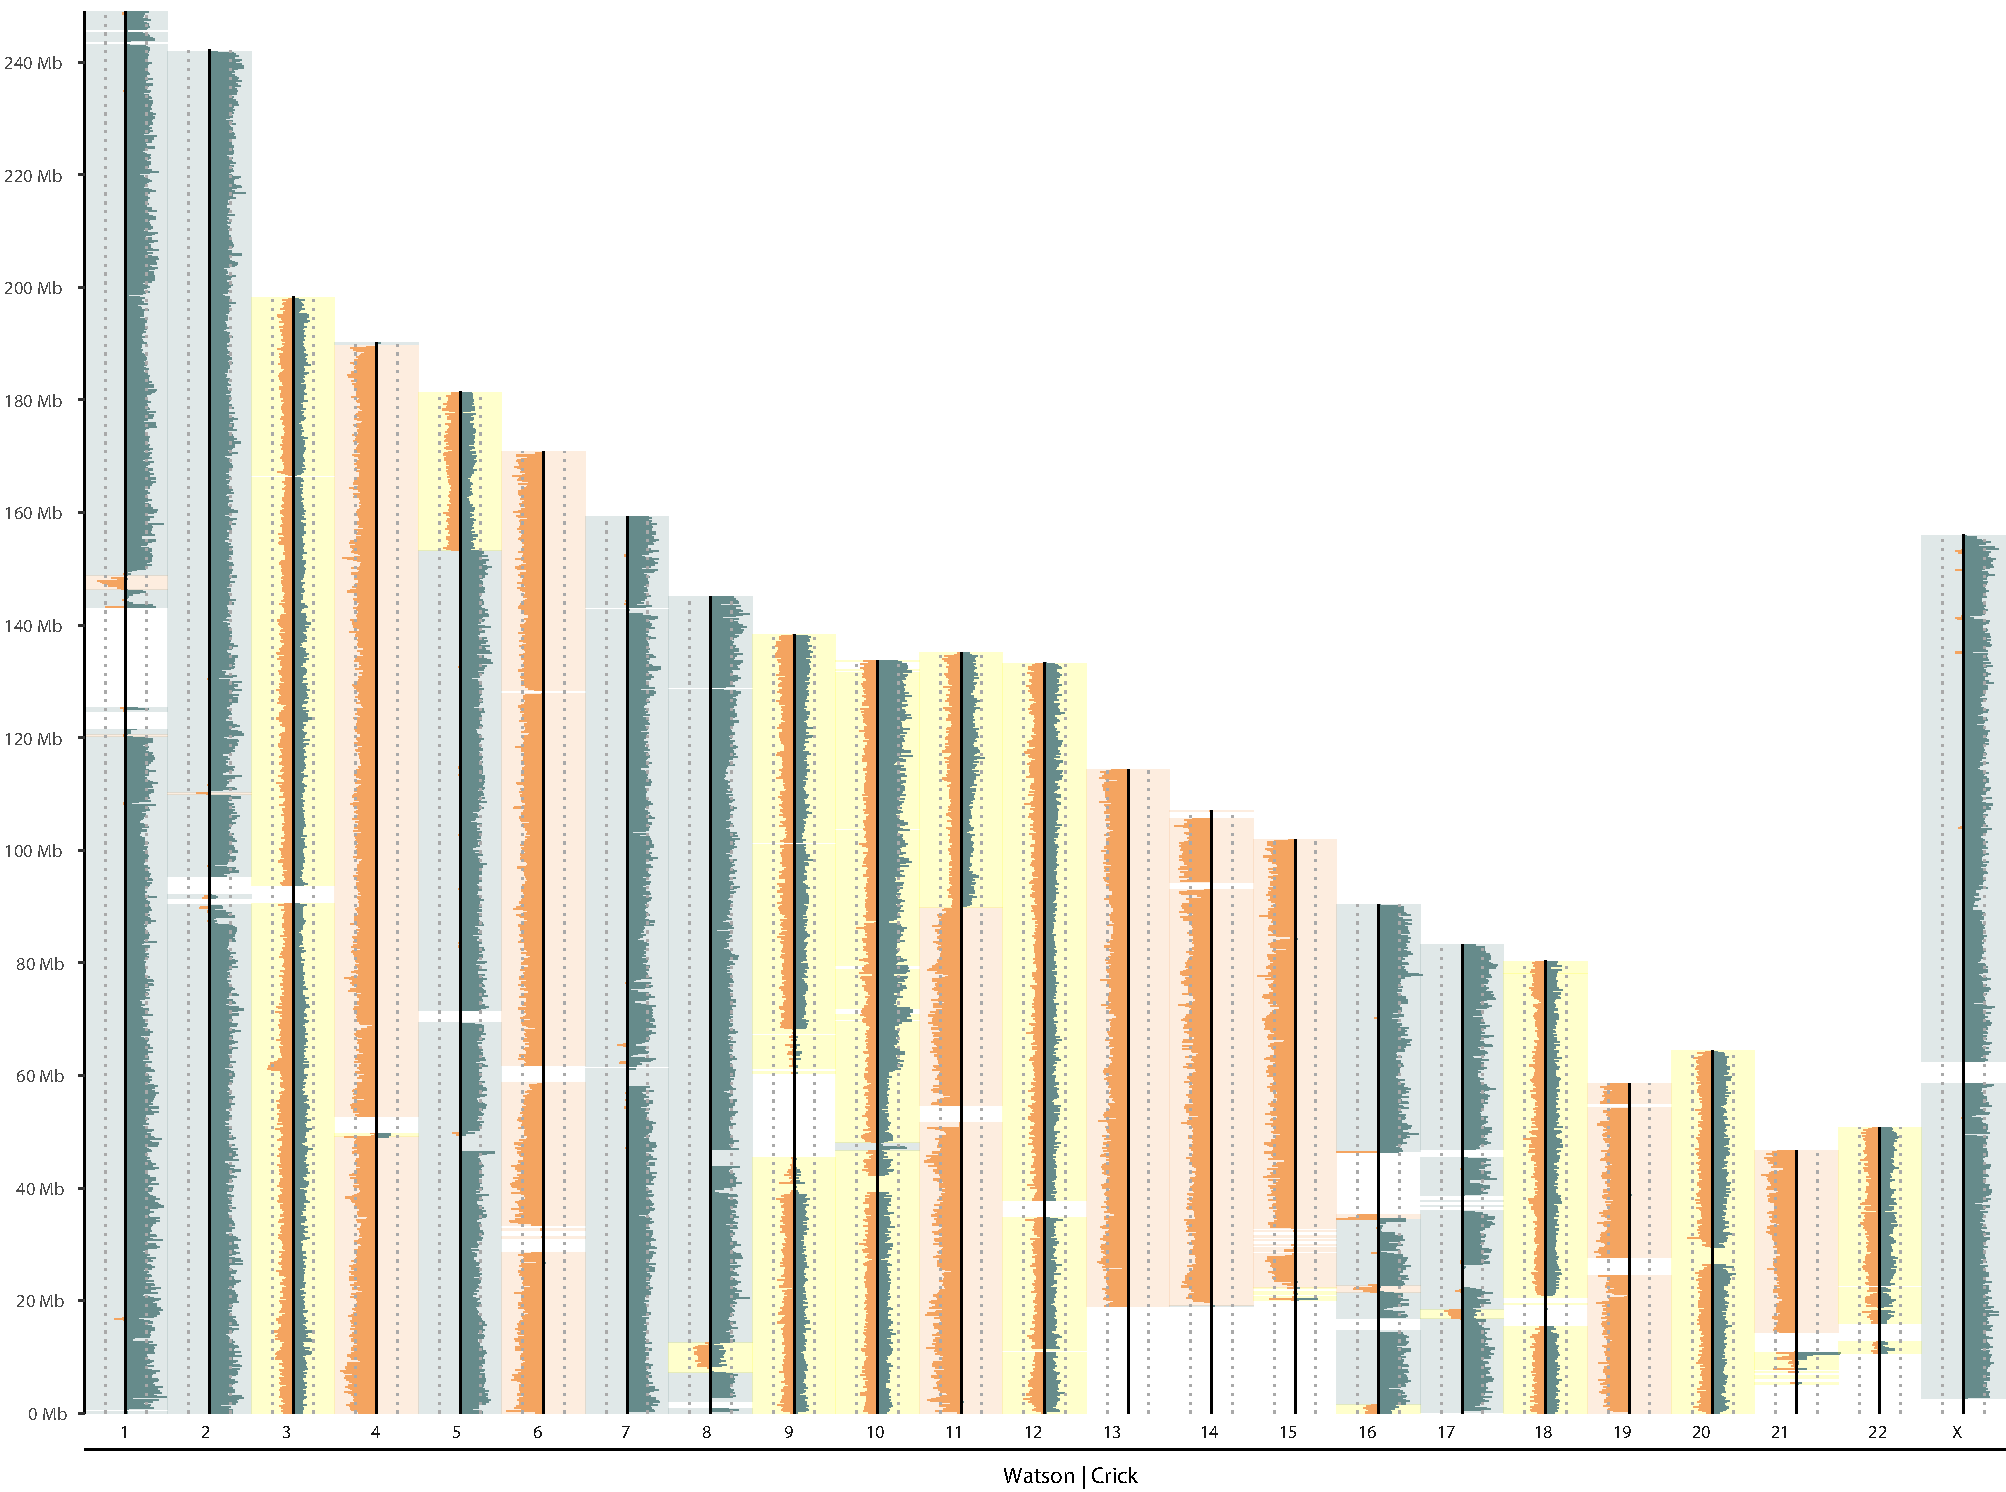
\includegraphics[width=\textplusmargin,inner]{ss_lib_rpewt.pdf}
        \figcap{ss_library}{Example of a single cell Strand-seq library}{
            Here, a single cell Strand-seq library of an \rpe-I wild type cell
            line is displayed using the plot function of \mc.
            Each vertical panel shows binned read counts of one chromosome, with
            the Watson strand on the left, in orange, and the Crick strand on
            the right in blue. In the cell shown here, each 200~kb-bin contains
            a median of 76 total reads, which is depicted by the
            dotted lines. Some regions, e.g. the centromere of chromosome 1 or
            the sub-telomeric regions of chromosomes 13--15 are not coverded by
            reads because of mappability issues; these bins are excluded from
            further analyses. The estimated strand inheritance state of each bin
            is color-coded in the background: blue for CC, orange for WW and yellow
            for WC. Chromosomes 5 and 11 carry \acp{sce}, which are visible by a
            change in the strand inheritance state that continues to the end of
            the chromosomes.}%
    \end{figure}
%    }}

\Cref{fig:ss_library} depicts Strand-seq data from a single cell of an \acf{rpe}
wild type cell line (courtesy by \balca and \landsdorp). This cell-wide overview
plot was generated using \mc and is typically the starting point for
an analysis of Strand-seq data. The procedure leading to this plot is outlined
briefly in \cref{sec:mosaic_method}.

An overview plot allows an initial judgment on the success, quality, and depth
of a Strand-seq library. In the cell shown here, reads aligning to either W or C
strand were binned at 200~kb resolution. The cell was sequenced at ample depth
(median 76 reads per bin), shows the Strand-seq characteristic strand
inheritance patterns (WW, CC, and WC chromosomes) and is of high quality, which
can be judged from the low number of reads on the opposite strand in WW or CC
cells and a fairly even coverage distribution. Experimental parameters
influencing the quality of Strand-seq libraries are discussed in detail by
\cite{Sanders2017}.

\Cref{fig:ss_library} further gives a first impression of genomic rearrangements
in this cell. For example, the region of WW reads at around 120~Mb on chromosome
1 reveals an inversion of that locus in respect to the reference assembly. The
most prominent alterations are visible on chromosomes 5 and 11, though. Here,
the strand inheritance states change at one position and remain consistent to
the end of the chromosome from there. These positions mark \acf{sce} events,
which are reciprocal exchanges between two identical sister chromatids and
which can be specifically measured using Strand-seq \citep{Falconer2012}.
\Acp{sce} occur randomly across the genome and must not be mistaken with other
classes of \acp{sv} for our purpose.





\subsection{Three signals within Strand-seq data are distinctive of SVs}
\label{sec:mosaic_concept}

Strand-seq libraries reveal the presence of large \Acl{sv}. This had been shown
for inversions in the past by \cite{Sanders2016}. Here, we determined seven
different \sv classes that can be revealed in Strand-seq data, five of which are
principally discernible within a single cell (deletion, duplication, inversion,
inverted duplication, \loh), and two that become apparent across a population of
cells (aneuploidy and translocation). These \sv classes can be distinguished
using three independent signals: (1) the normalized read coverage of a locus,
which corresponds to a diploid state (2N) in a non-affected locus.
(2) The strand ratio, i.e. the number of W reads over the number of C reads.
Alternatively, a fraction can be used here, for example the Watson fraction
W/(W+C). (3) Haplotype information. When whole-chromosome haplotypes are known
at sites of \acp{snv}, these alleles can be used to reason about potential
rearrangements. Sequencing reads overlapping such variants can be queried for
both their original homologue \emph{and} their strand direction.
Below I explain how we can utilize the combination of these signals to detect,
genotype and phase \acp{sv}. \Cref{fig:mosaic_examples} contains examples of
several \sv classes that we identified in \rpe cell lines.

\FloatBarrier
\begin{table}[t]%
\newcommand\ccb{\cellcolor{blue!10}}
\newcommand\cco{\cellcolor{orange!10}}
    \begin{adjustbox}{width=\textplusmargin,inner}%
    \begin{tabu} to \textplusmargin {X[l] c c c c l c c c c}
        \toprule
          & \multicolumn4{c}{WC chromosome} & & \multicolumn4{c}{WW chromosome} \\
         \cmidrule{2-5} \cmidrule{7-10}
          & & & \multicolumn2{c}{Haplotype} & & & & \multicolumn2{c}{Haplotype} \\
        \cmidrule(lr){4-5} \cmidrule(lr){9-10}
         & Cov. & W.f. & \emph{W} & \emph{C} & & Cov. & W.f. & \emph W & \emph{C} \\
        \midrule
        Reference allele             &      2N &      50\% & $h_1$   & $h_2$     & &      2N &      100\% & $h_1 + h_2$     & - \\
        Deletion of $h_1$            &      1N &       0\% & -       & $h_2$     & & \ccb 1N & \ccb 100\% & $h_2$           & - \\
        Deletion (homozygous)        &      0N &         - & -       & -         & &      0N &          - & -               & - \\
        Duplication of $h_1$         &      3N &      66\% & $2 h_1$ & $h_2$     & & \ccb 3N & \ccb 100\% & $2 h_1 + h_2$   & - \\
        Duplication (homozygous)     &      4N &      50\% & $2 h_1$ & $2 h_2$   & &      4N &      100\% & $2 h_1 + 2 h_2$ & - \\
        Inversion of $h_1$           &      2N &       0\% & -     & $h_1 + h_2$ & & \ccb 2N & \ccb  50\% & $h_2$ & $h_1$       \\
        Inversion (homozygous)       & \cco 2N & \cco 50\% & $h_2$   & $h_1$     & &      2N &        0\% & -     & $h_1 + h_2$ \\
        Inverted duplication ($h_1$) & \cco 3N & \cco 33\% & $h_1$ & $h_1 + h_2$ & & \ccb 3N & \ccb  66\% & $h_1 + h_2$ & $h_1$ \\
        \bottomrule
    \end{tabu}
    \end{adjustbox}
    \tabcap{mosaic_sv_signals}{Distinct signatures of focal SVs in Strand-seq
    data}{SVs can be identified based on three separate signatures of Strand-seq
    data: the total read coverage (\emph{Cov.}), the strand ratio---here shown
    as Watson fraction (\emph{W.f.}), and the presenece of haplotype-tagging
    \acp{snv} on each strand (\emph{Haplotpye}). In this table I show how the
    various focal \sv types can be inferred from these signals. This is different
    for WC chromosomes than for WW or CC chromosomes. For the sake of simpliciy,
    the table only shows the WW case and assumes heterozygous variants to affect
    haplotype $h_1$. Entries in orange are \sv classes that cannot be
    distinguished unambigously using only coverage and Watson fraction.
    Specifically, a homozygous inversions remain hidden in WC cells and an
    inverted duplication of $h_1$ cannot be distinguished from a duplication of
    $h_2$. Entries marked in blue cannot be phased based on coverage and Watson
    fraction alone. However, all these cases can be disentangled when
    haplotype-resolved \acp{snv} are available or by integrating information
    across several cells that share an \sv.}
\end{table}

\paragraph{Deletions and duplications}
\Acp{cnv} alter the total read coverage of an affected locus. A deletion
decreases the coverage from 2N to 1N, i.e. by a factor of two, and is hence
typically easier to detect---the same has been observed for other read
depth-based \sv callers. Duplications, which increase copy number to 3N, alter
the read depth only by a factor of 1.5 compared to the reference state.
Homozygous duplications increase the copy number even to 4N. Homozygous
deletions are marked by a complete absence of reads. They thus provide the
strongest change in read depth, with the only caveat that they resemble regions
of low mappability such as the centromere on chromosome 1. Homozygous deletions
are hence best studied in the presence of a control sample that does not carry
the deletion.

In contrast to classic read depth analysis, Strand-seq additionally provides
strand information. For example, a heterozygous deletion in a WC chromosome will
only lack reads on one of the strands. Similarly, a heterozygous duplication
will increase coverage only on one strand. In a WW or CC cell, strand
information does not add supportive evidence, but when phased \acp{snv} are
available, only one homologue will be deleted/duplicated.
\Cref{tab:mosaic_sv_signals} summarizes in detail how these signals
allow to differentiate the focal \sv classes that I cover here.

\paragraph{Copy-neutral variants}
Inversions do not change copy number, but become visible as a change in strand
ratio. A heterozygous inversion in a WW cell, for example, switches the strand
state to WC within the inverted locus. In a WC cell, it becomes WW or CC. Again,
in the WC cell the inversion can be phased trivially based on strand
directionality, whereas in the WW or CC case further \snv information has to be
consulted for phasing. A homozygous inversion is a special case: It changes a WW
chromosome into CC, making the locus clearly stand out, but it cannot be
observed within a WC cell. This is because both alleles change their strand
state, leading again to a WC region. This case can be disentangled with the help
of phased \acp{snv} or by observation of a population of cells
(\cref{tab:mosaic_sv_signals}).

Another copy-neutral \sv is \loh. In a \loh event, one homologue is
``overwritten'' by the other homologue, leading to extended regions of
homozygousity. To reveal \loh, alleles of\acp{snv} must be assessed. We recently
found independent regions of \loh within several cells of a lymphoblastoid cell
line (unbublished data)---all the work on haplotype information within this
project was spearheaded by \david and will hence not be covered in this
dissertation.

\paragraph{Complex variants}
Complex variants can partly be discovered in Strand-seq data, too. We chose
inverted duplications as a particular candidate, as this class has been found to
be abundant both on the small (\cref{sec:balancer}) as well as on the large
scale \citep{Chaisson2017}. As \cref{tab:mosaic_sv_signals} shows, inverted
duplications are marked by an increase in copy number as well as a flip in
strand orientation. In a WC cell, such an event cannot be distinguished from a
normal duplication unless \acp{snv} are available. \Cref{fig:mosaic_examples}
includes an example of an inverted duplication within an \rpe wild type cells.

\figuretextplusmargin[t!]{mosaic_sv_examples.pdf}{mosaic_examples}{Examples of SVs
    in RPE cells}{Strand-specific count data in 100~kb bins (Watson left, orange
    and Crick right, blue) are shown in several chromosomal regions of \rpe cells.
    \textbf{A:} Four loci of three cells each highlight four examples of focal
    \acp{sv} that could be identified in Strand-seq libraries. The affected
    loci (marked by dashed lines) show the characteristic changes in read
    coverage and strand state that were described in \cref{tab:mosaic_sv_signals}.
    \textbf{B:} A copy number gain of the q-arm of chromosome 10 is visible. The
    strand state of the extra copy correlates with the strand inheritance
    pattern of chromosome X (same cells for both chromosomes shown). This
    observation is best explained by an imbalanced translocation, as shown in
    the schematic.
    \textbf{C:} Five chromosomes of cells from the tetraploid RPE C29 cell line
    (courtesy by \balca and \landsdorp) were selected to represent the five
    possible strand inheritance patterns in a tetraploid cell: WWWW, WWWC, WWCC,
    WCCC, and CCCC.}


\paragraph{Aneuploidy}
In a Strand-seq experiment, each homologue of a chromosome is sequenced in
either W or C orientation. This fundamental property remains valid even in the
presence of more than two homologues. In a tetraploid cell, for example, a
chromosome is inherited in any one of five states: WWWW, WWWC, WWCC, WCCC, or
CCCC. By looking across a population of cells, Strand-seq can disclose the
ploidy of each chromosome, assuming it is not heterogeneous across cells
(\cref{fig:mosaic_examples}). A
usual way to estimate ploidy from \mps data is to assess the \baf of a bulk
sample---in a tetraploid chromosome, some \acp{snv} will be present at ratios of
25 or 75\%. Interestingly, Strand-seq detects ploidy even in the complete
absence of homologue-speicific variants, for example in cells with multiple
copies of the same homologue such as the CHM1 cell line \citep{Steinberg2014}.
To the best of our knowledge, this cannot be achieved by any other method.

\paragraph{Translocations}
At last, also translocations can be revealed using Strand-seq.  A reciprocal
translocation would alter the strand inheritance state of two chromosomes
simultaneously: An exchange between a WW and a CC chromosome would switch the
strand inheritance pattern into WC in both these chromosomes. However, such
changes in strand state can initially not be distinguished from randomly
occurring \sce events. This is why a correlated change between two chromosomes
must be observed across several cells to find translocations. In the \rpe wild
type cell line (\cref{fig:mosaic_examples}), we report an \emph{imbalanced}
translocation between chromosomes 10 and X, which had been noted
beforehand\footnote{In the description of the commercially available
    ``hTERT RPE-1'' cell line, a derivative of X is recognized, but chromosome
    10 is not mentioned. Source: \url{https://www.lgcstandards-atcc.org/Products/All/CRL-4000.aspx}}.
Here, chromosome 10 shows an increase in copy number on the q-arm that seems not
to be consistently on the same strand across cells. However, the strand
inheritance state of the extra copy perfectly matches the strand inheritance
state of chromosome X. This suggests that the extra copy of chromosome 10 is
linked physically to chromosome X. By correlating strand states across
chromosomes in this way, translocations can be discovered. The very same idea
has been used to assign unmapped contigs of the reference assembly to
chromosomes \citep{Hills2013}.







\FloatBarrier
\subsection{Automatd SV detecting}
\label{sec:mosaic_method}

In order to capture this spectrum of \sv classes, my collaborators and I
designed a computational approach for \sv calling from Strand-seq data.
This approach is implemented in a tool called \mc, which is currently being
developed. The core principle consists of the three steps (1) binning, (2)
segmentation, and (3) classification and is explained below. My code for the
first two steps is available online at
\url{https://github.com/friendsofstrandseq/mosaicatcher}.
The third part is being maintained by \maryam and can be found at
\url{https://github.com/friendsofstrandseq/MaRyam}. At last, the combined
workflow is available at \url{https://github.com/friendsofstrandseq/pipeline}.

\paragraph{Binning}
Strand-seq data is extremely sparse: the best libraries currently produced
contain around 300 reads per Megabases \citep{Chaisson2017,Sanders2017}. In
order to work with sparse data, I apply a binning scheme that summarizes
sequencing reads in windows of a given size, e.g. 50~kb. Alternatively, these
bins can have variable sizes (dynamic-width bins) to accommodate for regions of
low mappability. The transformation to binned counts allowed us to apply a
statistical model to estimate the expected number of reads per
bin---specifically, we utilized a \nb distribution, as I describe
later. Prior to binning, sequencing reads are filtered for low mapping quality
(a minimum score of 10 by default), supplementary alignments, and \pcr duplicates.
Also I only each read pair was counted only once to avoid double-counting of
sequenced fragments. I utilized the \htslib library within my implementation
to efficiently read and filter sequencing data.

Given the strand-specific binned counts, I implemented a plot function to
generate figures such as \cref{fig:ss_library}. At first, bins that are
consistently too low or high across all cells are masked: this is typically the
case in centromeric or telomeric regions. Further, I designed a classifier to
distinguish WW, WC, and CC states of each bin. This classifier is supposed to
tell the class of each bin based on its strand-specific read counts, but it
should further smoothen out fluctuations in single bins.
To achieve this, I implemented a \hmm with a multivariate \nb
emission distribution. The transition probability of the \hmm is chosen
according the expected number of \acp{sce} within a cell (e.g. 10 transitions
across all chromosomes). The output of this \hmm is used as background color in
aforementioned overview plots.

\paragraph{Segmentation}
The second step towards \sv calling is to detect the boundaries of potential
\acp{sv}. This had been done in the past by merging data of all cells in a
strand-aware fashion and detecting boundaries within the merged signal
\citep{Sanders2016}. However, this approach has the disadvantage that it can
mask subclonal variants, especially the ones at low allele frequency that we
are particularly interested in. Boundaries have also been determined within
single cells separately, e.g. based on an \hmm \citep{Bakker2016}. However, this
leads to the subsequent challenge of forming consensus boundaries across the
cells. Instead, I explored multivariate segmentation algorithms that consider
all cells simultaneously, yet still recognize them as individual cells. This is
further elaborated in \cref{sec:mosaic_segmentation}. Notably, the segmentation
algorithm is expected to provide potential \sv breakpoints, which are then
tested in the subsequent step. Thus, in order increase sensitivity, we allow the
segmentation to slightly overpredict boundaries.

\figurearbitrary[t!]{0.5}{mosaic_rpe_mean_var.pdf}{mean_var}{Mean variance
    relationship of binned read counts}{Each dot represents one cell of the
    \rpe-1 wild type cell line. Shown here are the mean number of reads per
    200~kb-bin vs. their variance. In a theoretical \nb distribution, mean and
    variance show a perfectly linear relationship with a slope $p$. In real data,
    we estimate $p$ by fitting a line without intercept.}

\paragraph{Classification} The third and final step is to test segments for the
presence of \acp{sv} (theory and implementation contributed by \maryam; figures
from me). In order to classify segments into either a \sv or non-\sv state, we
employ an elaborate Bayesian model based on \acl{nb} distributions.
Specifically, we model the read coverage in each strand by a \nb distribution,
which is adjusted to capture the expected number of reads within a given region.
Both strands combined yield a joint distribution for all possible strand
combinations, i.e. WW, WC, or CC, inclusing also abnormal states such as C, WWC,
and so on. Each of these joint strand states can then be interpreted in respect
to the expected state in the chromosome and cell. For example, a WC state would
signify a heterozygous inversion if it occurred on a WW chromosome, but no \sv
(or a homozygous inversion!) if it occurred on a WC chromosome.
\Cref{fig:nb_examples} gives a detailed example of how read counts are modeled
in a joint \nb distribution. The dispersion parameter of the \nb distribution,
$p$, is estimated across all cells, as \cref{fig:mean_var} explains. The second
\nb parameter controls the number of expected reads within a locus and must
hence be scaled to the size of the tested region. In line with our intuition,
a \nb distribution yields a clearer separation for higher counts, i.e. in larger
genomic regions intervals than for very small \acp{sv}. A shortcoming of our
approach is that the \nb distribution offers no intuitive way to model an
expectation of 0 counts, i.e. the absence of reads. We hence added a factor
$\alpha \approx 5\%$ to our model to formulate a \nb distribution that captures
zero counts. For instance, in a WW regions with $e$ expected total reads, the
expected number of C reads would be modeled by $\alpha \cdot e$ and the expected
number of W reads by $(1-\alpha) \cdot e$. In the end, the
estimated \nb probabilities for all \sv classes are considered across cells to
make a final decision about an \sv.

\figuretextplusmargin[t!]{NB_example.pdf}{nb_examples}{Graphical example of the
    negative binomial model}{The subplots on the top left and bottom right (in
    both panels) show the probability density functions of three \nb
    distributions. These distributions describe the probability of a given
    number of reads for the possible copy number states 0N, 1N, and 2N.
    In this example, the expected number of reads in a 2N state is 20 (blue
    curves). Both strands are modeled by separate \nb distributions, that, when
    combined, yield a joint probability (area of the rectangles).
    Here, only a the joint states W, C, WW, WC, CC are shown for the sake of
    simplicity (other possible states would be WWW, WWC, WWCC, and so on).
    In panel \emph{A}, 12 W and 8 C reads were observed, for which the joint
    strand state WC is by far the most likely one. In panel \emph{B}, 16 W and
    4 C were observed, which are best explained by a joint WW state, yet the
    difference to the runner up (WC) is not big.
    For SV calling, these joint states have to be interpreted in respect to the
    strand inheritance state of the chromosome: for example in a WC cell,
    example \emph{A} would be rejected (WC, i.e. reference, is the most likley
    state) but example \emph{B} would be considered for a heterozygous inversion
    (WW state).}

\paragraph{Additional steps}
Together with \maryam, \marschall and \david, we set up an automated workflow
with the aim to process Strand-seq data all the way from raw sequencing files to
final list of \sv predictions. This pipeline, which is based on the workflow
engine \snakemake, involves many other relevant steps in addition to the
tripartite calling procedure explained above, two of which shall be mentioned
here. First of all, the dominant strand state has to be determined for each cell
and chromosome in order to guide the \sv classification. This includes the
detection of \sce events. In order to achieve this, \venla implemented a
heuristic method to estimate strand states and \acp{sce} based on the output of
the strand state \hmm. This performed well when it was tested against experts'
opinions on real-world Strand-seq data. Secondly, haplotype information must be
annotated. \david hence incorporated functionality to annotate haplotypes in WC
chromosomes based on the \strandphaser tool. Interestingly, haplotype phasing
can be performed from Strand-seq data alone \citep{Porubsky2016}, which was also
built into the the workflow. With sufficient coverage, Strand-seq data can
even be used for \snv detection, which is a required input to phasing. Together,
this workflow supplies all input for subsequent \sv calling on Strand-seq data
without the requirement for additional data sets.





\subsection{A multivariate segmentation algorithm to find SV breakpoints}
\label{sec:mosaic_segmentation}

The objective of segmentation is to group the genome into consecutive regions of
the same copy number. This can be formulated as a problem of placing $k$
breakpoints in such a way, that the resulting consecutive segments best
represent a single copy number state each---the latter can be expressed in terms
of squarred (Gaussian) error. This problem gained much attention with the
availability of comparative genomic hybridization arrays to map \acp{cnv}.
Several methods were put forward for this task and a popular one is circular
binary segmentation \citep{Olshen2004,Venkatraman2007}. Today, these techniques
are also commonly applied to \mps data. The number of data points (hybridization
loci in arrays, or genomic bins in \mps experiments) critically impact the
runtime of such methods. Circular binary segmentation is efficient in this
respect, but it uses a heuristic approach (e.g. placing one breakpoint after the
other) that does not guarantee to find an optimal solution. In contrast, the
\textsc{tilingArray} \citep{Huber2006} package uses a dynamic programming
algorithm to find the optimal solution according to the squared error criterion.
As this algorithm does not scale well to deep \mps data, other approaches have
been proposed such as the Group fused LASSO formulation \citep{Bleakley2011}.

As Strand-seq data is inherently sparse, problem size is not a limitation factor
in our application. For example with 50~kb bins, chromosome 1 still only
contains \textasciitilde5000 data points. I hence designed and implemented an
algorithm for Strand-seq segmentation that is based on the \textsc{tilingArray}
principle\footnote{Original from \url{http://bioconductor.org/packages/release/bioc/html/tilingArray.html};
    implemented independently (including major changes) in \mc (see
    \texttt{segmentation.hpp})}.
The \textsc{tilingArray} algorithm internally uses a cost matrix that defines
how expensive (in terms of variance) each consecutive segment is. A dynamic
programming algorithm then choses the optimal combination of breakpoints. The
calculation of the cost matrix in \textsc{tilingArray} assumes the changes in
signal across all replicates to be the same, i.e. an increase at the same locus
in all samples. For Strand-seq data, I needed to relax this criterion to capture
inversions---where one strand is increased and another decreased---and mosaic
variation. I hence re-defined said cost matrix to allow individual jumps within
each strand. Notably, the positions of the breakpoints are still consistent
throughout all cells. I implemented this algorithm with all the bells and
whistles in \mc.




\FloatBarrier
\section{Simulation of Strand-seq data to explore the limits of \textsc{Mosaicatcher}}
\label{sec:mosaic_simul}

A principal challenge during the implementation of \mc was to measure its
performance. Initial results on \rpe cells looked very promising, but did not
allow a systematic investigation of the limitations of our method. In order to
make this possible, I developed a framework to simulate Strand-seq data.
Furthermore, the virtual Strand-seq cells can carry \acp{sv} in a fully
controlled manner. To give an example, \cref{fig:simulation_examples} shows
different simulated \sv classes at varying sizes. Naturally, such simulations
represent idealized conditions, yet they were designed in a way to closely
reflect essential properties of real-life data.
These simulations allow us to test the correctness of our method during the
development. More importantly though, they make it possible to explore the
theoretical limitations of \mc, e.g. in terms of the smallest SV size or lowest
variant frequency that can be detected reliably. Due to the
simulations we can focus our efforts on continously refining the methodology in
order to push these limits.



\subsection{Development of a versatile simulation framework}
\label{sec:mosaic_simul_framework}



\figurearbitrary[t!]{0.7}{mosaic_simulation_examples.png}{simulation_examples}{
    Examples of simulated \acp{sv} in different sizes}{The backgound data was
    simulated in 50~kb bins with a median of 20 reads per bin. \Acp{sv} were
    inserted at sizes of 100~kb, 400~kb, and 1~Mb and are highlighted by
    a blue background.}



\subsection{Assessing the performance of the segmentation algorithm}

\section{Conclusions and outlook}
\label{sec:mosaic_conclusion}



\chapter{Conclusions}
\label{sec:conclusions}

\section{Overview of findings}
\label{sec:findings}

The goal of this dissertation was to explore the potential of emerging DNA
sequencing technologies to discover, characterize and validate structural
variation. Throughout the projects described herein, I presented three concrete
use cases for this. Using emerging technologies I was able to scrutinize \acp{sv}
to an extent that had not been possible based on \mps. Importantly, the \acp{sv}
revealed by this led to novel insights into the complexity and functional role
of \acp{sv}. I also developed new computational approaches to detect and analyze
SVs based on these techniques which I make available to the community.

\paragraph{Complex inversions in the human genome}
In \cref{sec:complex_invs}, I analyzed inversions in the scope of the 1000
Genomes Project. Together with colleagues, we were able to solve the
``validation problem'' by using targeted long-read sequencing on both \pacbio
and \ont MinION platforms. I verified that more than 80\% of the predicted
inversions indeed carried an inversion signature---meaning they were
validated---which could previously be ascertained neither based on \mps data nor
via \pcr experiments. This solved my first research goal and a principal
challenge of the overall study \citep{Sudmant2015}.

Moreover, I then found that
the majority of predicted loci contained not simple inversions, but complex
variants containing inverted sequence. I categorized them into five major
classes, which included inverted duplications as the most frequent event. These
insights had only been possible due to the ability of long-read techniques to
span complete loci around predicted inversions. My analyses critically relied on
a visualization tool, which I developed simultaneously and which I made
available to the public (\url{https://github.com/dellytools/maze}).

The unforeseen amount of complex variation resulting from my work and the work
of others was one of the key lessons learned from the 1000 Genomes Project's \sv
study. The function and origin of these complex sv classes remained uncharted,
though. I thus carefully analyzed the breakpoints of complex \acp{sv} with the
goal to infer the mechanisms they originated from. The evidence I found was not
distinctive of any precise mechanism that might have formed these \acp{sv}, but
it suggested that several of the seemingly very different classes might
originate from the same mutagenic process. The work on complex variants has
since been continued and extended by others, further emphasizing the prevlanece
of this underappreciated phenomenon \citep{Collins2017}.

\paragraph{Effects of SVs on gene expression and chromatin organization}
In \cref{sec:balancer}, we had set out to study the functional consequences of
\acp{sv} in respect to gene expression and chromatin conformation. My first goal
within this collaborative project was to characterize the variants present in
highly rearranged balancer chromosomes. I achieved this by utilizing deep \wgs
and \hic data. Among many other aspects, I discovered the exact breakpoints of
large rearrangements of the balancer chromosomes. In the meantime, others had
mapped these breakpoints, too, and reassuringly, our results perfectly matched
their findings \citep{Miller2016,Miller2018}. However, through the technological
advantage of having \hic data, I could additionally detect precisely (in 2
cases) or approximately (in 1 case) the breakpoints that had been missed by
these studies. Further, I utilized haplotype-resolved \hic maps to validate
large rearrangements including a inversion and a duplication of 258~kb. The
large duplication most likely inserted in reverse orientation next to the
original copy, which I concluded from the differential contact frequencies
around the affected locus. Together, these findings clearly show the benefits
of \hic for the characterization of large \acp{sv}.

Afterwards, I implemented a
test for \acl{ase} that utilizes multiple biological replicates and that
corrects for effects of maternally deposited RNA. I found that changes in
expression occur almost everywhere across the genome and that they appear not to
be caused by enhancer hijacking, as had been observed in previous studies.
Instead, \acp{sv} alter expression via alternative mechanisms such as dosage
effects or chimeric expression of transcripts through mobile elements. Our
findings appear contrary to what has been seen in other scenarios; however, I
argue that this might be a result of natural selection in both these other
studies and in ours. Balancer chromosomes show a remarkable robustness towards
the huge rearrangements that they carry, and a potential enhancer hijacking
mechanism appears to be buffered. We think that these results will complement
previous studies and lead to a more holistic view on the role of chromatin
architecture. The manuscript was in preparation at the time of writing this
thesis.



\todo{more conclusions?}




\section{The impact of emerging sequencing technology on SV discovery}
\label{sec:impact}
\todo{whole section}



% Appendix
\appendix
\appendix


\clearpage
\phantomsection
\addcontentsline{toc}{part}{APPENDIX}
\part*{\Huge\bfseries\addfontfeature{LetterSpace=10}APPENDIX}
\label{sec:appendix}


\setcounter{chapter}{0}
\renewcommand\thechapter{\Alph{chapter}}


\small

\listofsoftware
\chapter{Supplementary information to \texorpdfstring{\cref{sec:complex_invs}}{the complex inversion project}}
\label{sec:suppl_inversions}



{
\tiny
\begin{longtable}{rrrlll}
    \tabcap{inversionlocilist}{Inversion loci resolved for breakpoint analysis}
           {These are the loci that could be resolved to nucleotide resolution
            with at least one of the three different approaches, namely Sanger
            sequencing, PacBio long-read assembly or Illumina short read
            assembly. Presented coordinates span the actual inversion.} \\
    \rule{0pt}{5ex} Chr & Start & End & Sample & SVtype & Source \\\hline \endfirsthead
    Chr & Start & End & Sample & SVtype & Source \\\hline \endhead
    1   & 2,810,097   & 2,813,130   & HG00240 & invdup  & Sanger  \\
    1   & 31,343,442  & 31,345,950  & NA18626 & invdup  & PacBio  \\
    1   & 44,821,288  & 44,824,322  & NA12717 & complex & PacBio  \\
    1   & 61,058,347  & 61,067,336  & pooled  & proxdup & Illumina  \\
    1   & 92,130,537  & 92,133,743  & NA12760 & simple  & PacBio  \\
    1   & 104,509,460 & 104,515,918 & pooled  & invdup  & Illumina  \\
    1   & 104,577,303 & 104,585,534 & NA19462 & invdup  & PacBio  \\
    1   & 115,678,410 & 115,684,369 & pooled  & proxdup & Illumina  \\
    1   & 116,117,516 & 116,124,785 & HG00683 & invdel2 & PacBio  \\
    1   & 118,866,376 & 118,875,456 & pooled  & proxdup & Illumina  \\
    1   & 119,491,847 & 119,494,184 & HG02187 & invdup  & PacBio  \\
    1   & 197,756,058 & 197,758,630 & HG01501 & simple  & PacBio  \\
    1   & 209,934,001 & 209,937,071 & NA19648 & proxdup & Sanger  \\
    1   & 225,093,501 & 225,096,376 & NA18952 & simple  & PacBio  \\
    1   & 232,812,220 & 232,815,483 & HG01488 & proxdup & Sanger  \\
    1   & 236,753,138 & 236,757,057 & NA19725 & invdup  & PacBio  \\
    1   & 240,115,049 & 240,118,193 & NA18909 & invdup  & PacBio  \\
    2   & 1,373,228   & 1,377,067   & HG01198 & proxdup & Sanger  \\
    2   & 38,523,662  & 38,527,434  & NA20862 & invdup  & PacBio  \\
    2   & 51,879,685  & 51,882,806  & NA20869 & invdup  & PacBio  \\
    2   & 61,699,968  & 61,704,838  & NA19908 & invdup  & PacBio  \\
    2   & 66,752,907  & 66,755,431  & NA20888 & invdup  & PacBio  \\
    2   & 72,066,684  & 72,069,956  & NA19462 & invdup  & PacBio  \\
    2   & 72,437,947  & 72,443,984  & HG01177 & invdup  & Sanger  \\
    2   & 77,048,694  & 77,054,125  & NA19440 & invdup  & PacBio  \\
    2   & 88,574,293  & 88,578,600  & NA12842 & complex & PacBio  \\
    2   & 100,816,898 & 100,819,370 & NA19130 & simple  & PacBio  \\
    2   & 125,765,562 & 125,769,408 & HG00260 & proxdup & Sanger  \\
    2   & 126,185,839 & 126,188,629 & HG01069 & proxdup & Sanger  \\
    2   & 129,683,821 & 129,687,475 & NA11919 & invdup  & PacBio  \\
    2   & 131,885,572 & 131,888,371 & HG01353 & invdup  & Sanger  \\
    2   & 133,517,218 & 133,520,825 & NA21104 & invdup  & PacBio  \\
    2   & 153,458,952 & 153,462,309 & NA20896 & invdel  & PacBio  \\
    2   & 176,681,072 & 176,689,113 & NA18621 & invdup  & PacBio  \\
    2   & 183,675,967 & 183,680,241 & HG02282 & invdup  & PacBio  \\
    2   & 187,155,554 & 187,158,547 & HG00261 & invdel  & PacBio  \\
    2   & 216,826,684 & 216,829,198 & NA19716 & simple  & PacBio  \\
    2   & 226,994,897 & 227,002,679 & HG01464 & proxdup & Sanger  \\
    2   & 230,842,479 & 230,846,050 & NA21123 & invdup  & PacBio  \\
    3   & 10,738,894  & 10,741,904  & NA18597 & invdup  & PacBio  \\
    3   & 12,988,206  & 12,991,165  & HG01191 & invdup  & Sanger  \\
    3   & 18,655,279  & 18,658,136  & NA19256 & complex & PacBio  \\
    3   & 36,405,643  & 36,408,059  & NA20813 & simple  & PacBio  \\
    3   & 43,834,099  & 43,837,000  & NA12763 & invdup  & Sanger  \\
    3   & 88,545,013  & 88,552,419  & pooled  & proxdup & Illumina  \\
    3   & 104,030,235 & 104,039,365 & HG01710 & complex & PacBio  \\
    3   & 122,889,782 & 122,893,062 & NA19663 & invdup  & PacBio  \\
    3   & 127,495,514 & 127,498,977 & NA18909 & invdup  & PacBio  \\
    3   & 133,687,260 & 133,690,830 & HG02568 & invdup  & PacBio  \\
    3   & 139,978,284 & 139,981,411 & NA12750 & proxdup & Sanger  \\
    3   & 160,277,732 & 160,279,909 & NA20890 & invdup  & PacBio  \\
    3   & 165,030,799 & 165,033,479 & NA19701 & invdup  & PacBio  \\
    3   & 168,104,732 & 168,106,843 & HG02081 & invdup  & PacBio  \\
    3   & 184,308,171 & 184,311,964 & NA18993 & complex & PacBio  \\
    3   & 190,832,762 & 190,835,088 & NA18877 & invdup  & PacBio  \\
    3   & 196,276,818 & 196,280,716 & NA19375 & complex & PacBio  \\
    4   & 16,916,389  & 16,918,472  & HG01610 & invdel  & PacBio  \\
    4   & 23,127,395  & 23,133,886  & HG01105 & proxdup & Sanger  \\
    4   & 26,485,682  & 26,488,207  & NA20766 & simple  & PacBio  \\
    4   & 45,755,433  & 45,758,093  & HG02508 & invdel2 & PacBio  \\
    4   & 53,703,955  & 53,706,001  & NA19213 & invdup  & PacBio  \\
    4   & 62,473,294  & 62,477,236  & NA12717 & invdel  & PacBio  \\
    4   & 83,860,778  & 83,864,528  & NA19703 & invdel2 & PacBio  \\
    4   & 101,598,859 & 101,602,434 & NA18498 & invdel  & PacBio  \\
    4   & 110,134,019 & 110,138,014 & NA18621 & simple  & PacBio  \\
    4   & 112,006,211 & 112,009,195 & NA20506 & invdup  & PacBio  \\
    4   & 115,289,789 & 115,293,034 & NA19429 & invdup  & PacBio  \\
    4   & 117,788,673 & 117,791,591 & NA19652 & invdel2 & PacBio  \\
    4   & 120,584,771 & 120,588,111 & NA19117 & invdup  & PacBio  \\
    4   & 138,659,437 & 138,661,397 & NA19380 & simple  & PacBio  \\
    4   & 148,548,181 & 148,555,509 & NA12155 & invdup  & PacBio  \\
    4   & 151,163,095 & 151,167,180 & HG00120 & proxdup & Sanger  \\
    5   & 10,905,194  & 10,909,204  & NA12878 & invdup  & PacBio  \\
    5   & 18,083,693  & 18,087,591  & HG01510 & invdel  & PacBio  \\
    5   & 31,189,246  & 31,194,091  & pooled  & invdup  & Illumina  \\
    5   & 32,884,289  & 32,887,629  & NA20815 & simple  & PacBio  \\
    5   & 92,760,283  & 92,763,153  & NA20298 & invdup  & PacBio  \\
    5   & 95,599,929  & 95,602,938  & HG02008 & invdup  & PacBio  \\
    5   & 116,049,680 & 116,052,708 & NA19457 & invdup  & PacBio  \\
    5   & 128,383,831 & 128,388,265 & pooled  & invdup  & Illumina  \\
    5   & 142,283,542 & 142,286,903 & NA19401 & invdup  & PacBio  \\
    5   & 143,511,483 & 143,516,048 & NA19429 & proxdup & Sanger  \\
    5   & 167,176,735 & 167,179,485 & HG00132 & invdup  & PacBio  \\
    5   & 171,074,258 & 171,077,635 & NA19404 & simple  & PacBio  \\
    5   & 171,845,749 & 171,848,814 & NA19334 & invdup  & PacBio  \\
    5   & 174,875,526 & 174,878,773 & HG03162 & invdup  & PacBio  \\
    5   & 174,891,963 & 174,895,522 & NA21120 & invdel  & PacBio  \\
    5   & 178,122,463 & 178,126,334 & NA18552 & invdel  & PacBio  \\
    6   & 341,808     & 345,233     & HG03052 & proxdup & Sanger  \\
    6   & 3,883,917   & 3,888,364   & NA18519 & invdel  & PacBio  \\
    6   & 12,435,664  & 12,442,395  & pooled  & invdup  & Illumina  \\
    6   & 22,949,565  & 22,952,564  & HG02178 & simple  & PacBio  \\
    6   & 24,044,152  & 24,046,232  & NA18528 & simple  & PacBio  \\
    6   & 32,314,159  & 32,317,262  & HG00102 & proxdup & Sanger  \\
    6   & 32,980,439  & 32,986,191  & pooled  & proxdup & Illumina  \\
    6   & 41,039,563  & 41,047,733  & pooled  & proxdup & Illumina  \\
    6   & 91,942,170  & 91,951,265  & pooled  & proxdup & Illumina  \\
    6   & 119,010,711 & 119,014,924 & HG01879 & proxdup & Sanger  \\
    6   & 119,539,622 & 119,543,304 & NA12348 & simple  & PacBio  \\
    6   & 138,060,160 & 138,062,315 & HG00554 & invdel  & PacBio  \\
    7   & 811,112     & 813,724     & NA19451 & invdup  & PacBio  \\
    7   & 3,488,490   & 3,491,579   & HG01083 & invdup  & PacBio  \\
    7   & 8,350,680   & 8,358,342   & NA20845 & invdel  & PacBio  \\
    7   & 18,724,936  & 18,730,404  & HG02943 & invdup  & PacBio  \\
    7   & 25,683,658  & 25,686,303  & NA20876 & invdup  & PacBio  \\
    7   & 30,507,209  & 30,513,004  & pooled  & proxdup & Illumina  \\
    7   & 38,233,698  & 38,238,284  & NA19119 & invdup  & PacBio  \\
    7   & 50,263,289  & 50,266,539  & NA18596 & invdup  & PacBio  \\
    7   & 53,018,261  & 53,028,101  & NA10847 & invdup  & Sanger  \\
    7   & 90,062,875  & 90,071,654  & HG03367 & invdup  & PacBio  \\
    7   & 101,637,967 & 101,642,114 & NA19383 & invdel2 & PacBio  \\
    7   & 117,008,274 & 117,015,041 & HG00683 & invdup  & PacBio  \\
    7   & 127,202,018 & 127,206,098 & NA12760 & proxdup & Sanger  \\
    7   & 128,817,901 & 128,821,861 & NA19213 & invdup  & PacBio  \\
    7   & 139,979,709 & 139,986,651 & NA20521 & invdel  & PacBio  \\
    7   & 151,009,481 & 151,013,242 & NA19716 & invdup  & PacBio  \\
    8   & 21,307,540  & 21,312,322  & pooled  & proxdup & Illumina  \\
    8   & 26,348,722  & 26,351,695  & NA19116 & invdup  & PacBio  \\
    8   & 43,285,112  & 43,288,081  & HG00565 & invdup  & PacBio  \\
    8   & 47,500,475  & 47,503,744  & NA12717 & proxdup & Sanger  \\
    8   & 80,510,952  & 80,515,416  & NA19393 & complex & PacBio  \\
    8   & 87,669,453  & 87,673,747  & NA19099 & complex & PacBio  \\
    8   & 100,156,890 & 100,159,093 & NA18596 & invdup  & PacBio  \\
    8   & 103,891,670 & 103,894,247 & NA19372 & simple  & PacBio  \\
    8   & 110,096,523 & 110,100,023 & NA20528 & invdup  & PacBio  \\
    8   & 117,091,416 & 117,096,195 & HG01595 & invdup  & Sanger  \\
    8   & 122,512,509 & 122,516,193 & NA21089 & invdup  & PacBio  \\
    8   & 133,531,442 & 133,535,173 & HG01190 & proxdup & Sanger  \\
    8   & 135,239,332 & 135,242,167 & NA18621 & invdup  & PacBio  \\
    8   & 138,129,967 & 138,132,573 & NA12812 & invdup  & Sanger  \\
    8   & 138,347,078 & 138,350,618 & NA12878 & invdup  & PacBio  \\
    9   & 15,127,054  & 15,129,637  & HG02946 & invdup  & PacBio  \\
    9   & 20,075,503  & 20,081,530  & pooled  & proxdup & Illumina  \\
    9   & 34,595,327  & 34,601,065  & HG03052 & invdup  & PacBio  \\
    9   & 38,666,722  & 38,675,128  & pooled  & invdup  & Illumina  \\
    9   & 79,778,313  & 79,781,868  & NA19314 & invdup  & PacBio  \\
    9   & 87,133,944  & 87,139,287  & pooled  & invdup  & Illumina  \\
    9   & 88,741,878  & 88,745,736  & NA19720 & invdel  & PacBio  \\
    9   & 91,735,559  & 91,739,219  & NA20757 & invdup  & PacBio  \\
    9   & 94,720,336  & 94,722,969  & NA19466 & simple  & PacBio  \\
    9   & 125,378,010 & 125,381,471 & NA19307 & invdup  & PacBio  \\
    9   & 125,484,055 & 125,492,389 & NA19312 & invdup  & PacBio  \\
    9   & 134,394,191 & 134,398,761 & HG02035 & invdup  & PacBio  \\
    10  & 62,063,542  & 62,065,680  & NA19684 & invdel  & PacBio  \\
    10  & 76,503,187  & 76,506,726  & NA19661 & invdup  & PacBio  \\
    10  & 77,858,287  & 77,861,697  & HG03304 & simple  & PacBio  \\
    10  & 86,799,703  & 86,804,886  & pooled  & proxdup & Illumina  \\
    10  & 87,242,251  & 87,246,132  & NA19920 & complex & PacBio  \\
    10  & 97,205,777  & 97,209,023  & NA19397 & proxdup & Sanger  \\
    10  & 99,778,760  & 99,783,080  & NA18636 & simple  & PacBio  \\
    10  & 107,247,393 & 107,251,563 & NA19088 & invdup  & PacBio  \\
    10  & 115,014,501 & 115,018,805 & pooled  & proxdup & Illumina  \\
    10  & 115,170,837 & 115,172,953 & NA19701 & simple  & PacBio  \\
    11  & 24,902,559  & 24,905,575  & NA19093 & invdup  & PacBio  \\
    11  & 25,353,203  & 25,361,606  & pooled  & proxdup & Illumina  \\
    11  & 66,017,849  & 66,020,965  & NA20852 & invdel  & PacBio  \\
    11  & 73,475,246  & 73,484,209  & HG03115 & invdup  & PacBio  \\
    11  & 105,571,092 & 105,576,377 & NA19655 & complex & PacBio  \\
    11  & 113,803,414 & 113,808,661 & pooled  & proxdup & Illumina  \\
    11  & 131,064,693 & 131,067,736 & NA19114 & invdup  & PacBio  \\
    12  & 24,294,074  & 24,296,700  & NA19700 & simple  & PacBio  \\
    12  & 26,988,940  & 26,992,947  & NA19920 & simple  & PacBio  \\
    12  & 38,316,933  & 38,320,034  & HG01992 & invdup  & PacBio  \\
    12  & 45,744,570  & 45,752,672  & pooled  & proxdup & Illumina  \\
    12  & 51,996,881  & 52,000,148  & NA19152 & simple  & PacBio  \\
    12  & 71,707,228  & 71,712,753  & NA06994 & invdup  & PacBio  \\
    12  & 78,382,870  & 78,389,248  & NA12005 & invdup  & Sanger  \\
    12  & 91,377,082  & 91,383,619  & pooled  & invdup  & Illumina  \\
    12  & 94,337,361  & 94,347,985  & pooled  & proxdup & Illumina  \\
    12  & 95,333,304  & 95,335,398  & HG02017 & invdup  & PacBio  \\
    12  & 95,951,781  & 95,954,935  & NA19712 & invdup  & PacBio  \\
    12  & 117,588,989 & 117,591,059 & NA18570 & invdup  & PacBio  \\
    12  & 121,338,020 & 121,340,751 & HG03367 & invdup  & PacBio  \\
    13  & 25,801,807  & 25,804,767  & NA18489 & invdel  & PacBio  \\
    13  & 40,172,270  & 40,176,559  & NA12340 & invdup  & PacBio  \\
    13  & 44,679,673  & 44,682,428  & NA19062 & simple  & PacBio  \\
    13  & 74,690,142  & 74,692,748  & NA18870 & invdup  & PacBio  \\
    13  & 103,199,207 & 103,204,904 & HG01085 & invdup  & PacBio  \\
    14  & 25,610,038  & 25,615,609  & NA11994 & invdel2 & PacBio  \\
    14  & 44,689,839  & 44,692,672  & HG00419 & simple  & PacBio  \\
    14  & 48,323,276  & 48,325,817  & NA19719 & invdup  & PacBio  \\
    14  & 50,461,714  & 50,467,254  & NA18567 & invdup  & PacBio  \\
    14  & 54,420,845  & 54,423,480  & NA18559 & simple  & PacBio  \\
    14  & 59,039,358  & 59,042,736  & NA19457 & invdel2 & PacBio  \\
    14  & 62,255,009  & 62,258,710  & NA21091 & invdup  & PacBio  \\
    14  & 65,841,159  & 65,843,994  & NA20525 & invdel  & PacBio  \\
    15  & 38,482,819  & 38,490,047  & NA18563 & invdup  & PacBio  \\
    15  & 46,052,726  & 46,055,399  & HG01365 & invdup  & PacBio  \\
    15  & 68,406,025  & 68,409,036  & HG01051 & invdup  & Sanger  \\
    16  & 55,917,832  & 55,921,409  & NA19462 & invdel  & PacBio  \\
    16  & 69,179,664  & 69,182,488  & NA18552 & invdel  & PacBio  \\
    16  & 69,759,566  & 69,765,483  & pooled  & invdup  & Illumina  \\
    16  & 78,036,292  & 78,043,806  & pooled  & proxdup & Illumina  \\
    17  & 26,112,410  & 26,115,025  & NA18916 & simple  & PacBio  \\
    17  & 33,180,764  & 33,183,545  & HG01776 & invdup  & PacBio  \\
    17  & 40,541,067  & 40,546,253  & NA18563 & invdel  & PacBio  \\
    17  & 46,614,626  & 46,618,231  & HG01334 & proxdup & Sanger  \\
    17  & 64,938,572  & 64,944,951  & pooled  & proxdup & Illumina  \\
    17  & 76,845,394  & 76,849,002  & NA19319 & simple  & PacBio  \\
    18  & 13,917,343  & 13,920,817  & NA18879 & invdup  & PacBio  \\
    18  & 39,837,841  & 39,841,521  & HG00266 & invdup  & PacBio  \\
    18  & 69,710,794  & 69,713,885  & HG00268 & proxdup & Sanger  \\
    18  & 73,931,872  & 73,939,922  & pooled  & proxdup & Illumina  \\
    19  & 41,138,443  & 41,146,725  & HG02938 & invdup  & PacBio  \\
    20  & 2,358,695   & 2,361,666   & HG00246 & proxdup & Sanger  \\
    20  & 43,963,732  & 43,966,725  & NA19393 & invdup  & PacBio  \\
    20  & 58,306,804  & 58,309,850  & NA18944 & simple  & PacBio  \\
    21  & 20,646,874  & 20,649,790  & NA11832 & complex & PacBio  \\
    21  & 43,343,620  & 43,352,881  & NA18635 & simple  & PacBio  \\
    X   & 18,606,738  & 18,611,680  & HG01625 & invdup  & PacBio  \\
    \end{longtable}
}

\chapter{Supplementary information to \texorpdfstring{\cref{sec:balancer}}{the balancer project}}
\label{sec:suppl_balancer}


The content of this supplementary chapter is largly taken from the supplementary
methods in \textbf{our paper}\todo{cite our paper} and partly adapted when
neccessary.

\section{SNV calling}
\label{sec:suppl_snv}

Both \wgs and mate pair sequencing data was mapped to
\ac{dm6} using \bwamem version 0.7.15. \Ac{snv} and short indel calling was
performed using \freebayes version v0.9.21-19 with disabled population priors on
the \wgs data of both $F_0$ and $F_1$ samples simultaneously. The results were
filtered using \vcflib based on a quality value of at least 30,
a minimum of at least two reads carrying the allele to the right and to the left
end, and on the fact that the allele was seen on at least two reads mapping in
each direction. We further normalized variants, removed mutli-allelic variants,
and decomposed multi-nucleotide substitutions (which are reported as haplotype
blocks by \freebayes) into \acp{snv} using \vt (the sub-command \textsc{decompose\_blocksub}
was used for decomposition). We finally remove contigs other than chromosome 2,
3, and X and obtained a total of 860,095 \acp{snv} and small indels.



\section{Mutational signature analysis}
\label{sec:suppl_mutsign}

Starting from the set of 520,521 balancer- or wild type-specific \acp{snv},
I removed the ones which are present in the DGRP freeze 2.0 \snv call set.
Then I used the R package \textsc{SomaticSignatures} \citep{Gehring2015} to
count base substitutions and their contexts of the remaining 58,457 variants
and plotted their relative frequencies in \cref{fig:signatures}. The absence
of striking differences between balancer and wild type spectra demotivated me
from deeper investigations of mutational signatures.

\figuretextplusmargin{snp_signatures_dgrp_removed.pdf}
    {signatures}
    {\Ac{snv} mutation spectrum}
    {Frequency of the different
     base substitutions in their three-nucleotide context for balancer- and
     wild type-specific \acp{snv}. \Acp{snv} that are found in DGRP were
     removed, leaving 58,457 variants.}




\section{Deletion calling}
\label{sec:suppl_del}

I used \delly version 0.7.2 on the \wgs data of the $F_0$ and $F_1$ data
simultaneously and applied an extensive filtering procedure to reduce the number
of false positive calls. From the initial 10,421 deletion calls, 5,150 dropped
out because they were not flagged as ``QC PASS'', were not on one of the main
chromosomes (\ac{chr2}, \ac{chr3}, or \ac{chrX}), had a mapping quality value of
less than 60 or did not match the expected genotypes (i.e. balancer-specific,
wild type-specific, and common - together constituting more than 90\% of the calls).
Furthermore I required a minimum number of supporting read pairs for reference
and alternative allele combined, namely 40 read pairs for ``imprecise'' \delly
calls and 25 split reads for breakpoint-precise \delly calls.

Next, I developed a dynamic read depth ratio filter that was applied to deletion
predictions of 160~bp or larger.
To this end, the read count within the predicted deletion was normalized by the
summed read count in size-matched intervals flanking the locus and these values
were compared between samples. I required a minimum difference in the read depth
ratio between samples with different genotypes and this threshold increases
dynamically with \sv size. This is motivated by the fact that for larger deletions
the average read depth signal is more robust against local fluctuations in coverage.
To give an example, this filter removed a number of predictions above 100~kb in
size, which could be clearly identified as false positives by inspecting additional
(e.g. Hi-C) data. At last I overlapped deletions with a mappability map to
classify them into high (at least 50\% in a uniquely mappable region) or
low-confidence loci. Eventually we obtained four call sets: 3,072 calls with
high-confidence and below 50~bp, 737 calls with high confidence and from
50~-~159~bp, 395 large calls with high confidence and 75 large ones with low
confidence.

As a validation \yad performed \pcr on randomly selected loci in the latter three
categories. I designed primers using a lab-internal extension to \primerthree
and \yad amplified 25 loci per category in both samples via \pcr.
In the size range 50-159~bp 24 out of 25 loci validated, also 24/25 loci
validated for high confidence calls of 160~bp, and 25/25 loci validated for
low-confidence calls, yielding an estimated FDR of 2.66\%.
At last we merged the set of \delly deletion calls into the set of small
deletions called by \freebayes and chose a lower size cutoff of 15~bp. During
the merging process \freebayes calls were given priority over matching \delly
calls (based on 50\% reciprocal overlap). The final data set (referred to as
``deletions'' in the main text) contains 8,340 deletions on chromosomes 2, 3 and
X.




\section{Duplication calling and filtering}
\label{sec:suppl_dup}

\figuretextwidth{dup_validation_example_wt.pdf}{dup_validation_wt} % DUP00014221
    {Example for a wild type-specific duplication}
    {Wild-type specific tandem duplication at locus
    \textit{chr3R:26,960,008−26,964,205}. The bi-allelic frequnency signal
    clearly suggests a heterozygous duplication in the $F_1$ cross and the
    increased read depth in the wild type sample identifies it as present on
    the wild type chromosome.}

\figuretextwidth{dup_validation_example_false.pdf}{dup_validation_false} %
    {Example for a false duplication prediction}
    {Predicted duplication locus \textit{chr3R:22,101,264−22,107,086} is not
    validated by the bi-allelic frequncy signal.}

I used \delly version 0.7.5 in tandem duplication mode and supplied both mate
pair and \wgs libraries for $F_0$ and $F_1$ samples simultaneously. Duplication
calls were initially filtered by the ``quality PASS'' criteria reported by
\delly and by their combined genotypes, which were required to be heterozygous
in the $F_1$ sample. We do not require homozygosity in the $F_0$ sample due to a
known issue of the duplication classifier, which reports many homozygous tandem
duplications as heterozygous. For all remaining 352 calls I generated detailed
overview plots that contained multiple lines of information: a total read-depth
track, a mappability track, overlapping gene annotations and, importantly, a
track showing the bi-allelic frequency measured at SNV positions. These plots
allowed me to sort out false positives, leaving 122 manually curated
high-quality tandem duplications. Aside from tandem duplications I further
inspected the bi-allelic frequency ratio across the genomes and unraveled three
non-tandem duplications of 4.3~kb, 10.4~kb and 258~kb size. Both sets together
are summarized by ``duplications'' in the main text.


\listofreferences

\end{document}
